\documentclass[a4paper]{article}
\usepackage[utf8]{inputenc}
\title{Rapport BE Automatique}
\author{Nicolaï BEUHORRY-SASSUS - Quentin POINTEAU}
\date{}

\usepackage{amsmath}    % Pour des maths
\usepackage{amssymb}    % Pour des maths
\usepackage{stmaryrd}   % Pour des maths
\usepackage{graphicx}   % Pour inclure des images
\usepackage{fullpage}
\usepackage{caption}
\usepackage{subcaption} % Pour les subfigures
\usepackage{fancyhdr}   % Pour les en-têtes et pieds de pages personnalisés
\usepackage{lastpage}   % Pour obtenir le numéro de la dernière page
\usepackage{minted}     % Pour l'incorporation de code

\pagestyle{fancy}
\lhead{}
\chead{}
\rhead{}
\lfoot{ENSEEIHT - 1A SN}
\cfoot{}
\rfoot{Page \thepage/\pageref{LastPage}}
\renewcommand{\headrulewidth}{0pt}
\renewcommand{\footrulewidth}{0pt}

\setlength{\parindent}{0pt}     % Mettre l'indentation automatique à 0pt

\DeclareMathOperator{\tr}{tr}   % Définir l'opérateur mathématique trace

\begin{document}
        \maketitle
        \tableofcontents
        \listoffigures
        \listoftables
        \vspace{20pt}

        \hspace{25pt} Ce bureau d'étude a eu pour objectif, en lien avec le cours et les tds, de nous initier à la théorie des sytèmes 
        au travers de différentes notions fondamentales parmis lesquelles on retrouve : la théorie du contrôle, les systèmes 
        commandées, la stabilité des systèmes dynamiques ou encore la commande des systèmes cyber-physique qui inclue elle-même 
        la contrôlabilité, l'observabilité et la stabilisation par retour d'état. Tout au long de ce parcours, nous avons 
        utilisé comme objet d'étude le \textit{Robot Lego Segway}, qui nous a permi entre autres de visualiser et mettre en 
        application toutes les connaissances transmises. Ainsi, nous allons retracer au travers de ce rapport, en mentionnant 
        succinctement les notions nécéssaires à la compréhension, la démarche que nous avons suivie pour satisfaire l'exigence 
        suivante qui était de stabiliser à la verticale et à l'arrêt le \textit{Robot Lego Segway}.

        \begin{figure}[h!]
                \centering
                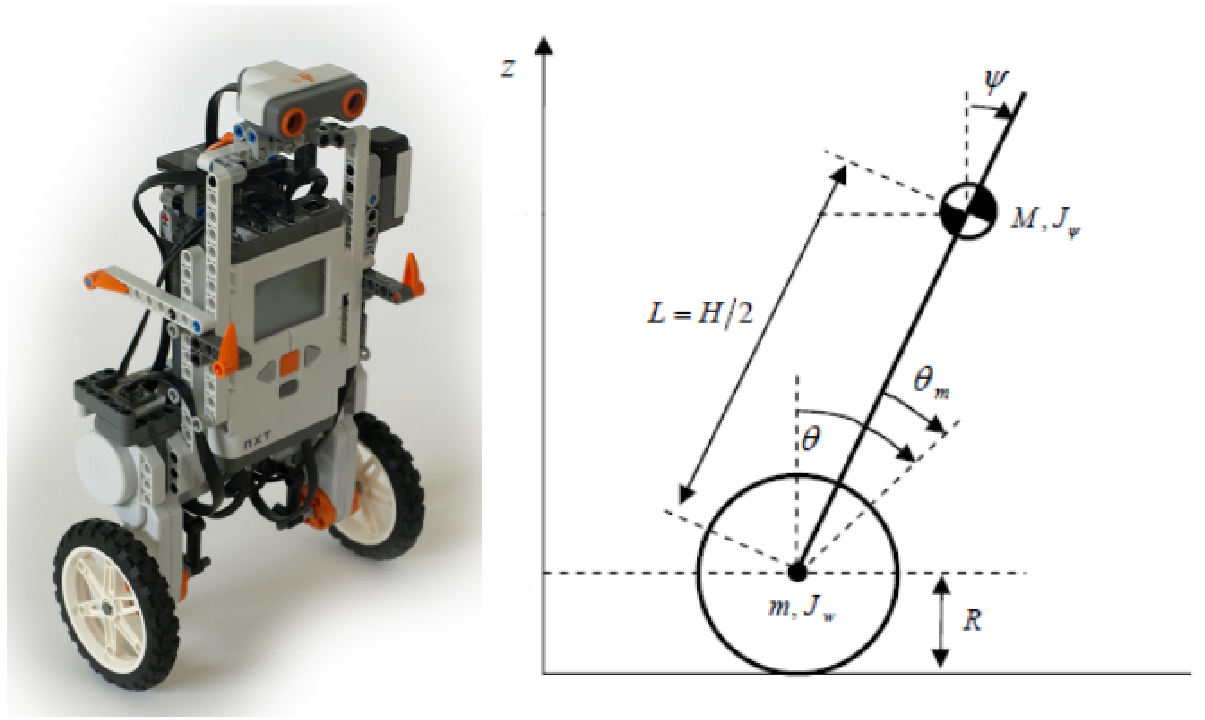
\includegraphics[scale=0.25]{images/robot_lego.png}
                \caption{Illustration du Robot Lego Segway ainsi que sa schématisation}
                \label{fig_robot_lego}
        \end{figure}


        \section{Positionnement du problème}

                Une première étape consiste à décrire à l'aide d'équations physiques le comportement du système.
                Pour ce faire nous allons dans une première partie assimiler le fonctionnement du robot à l'arrêt à celui d'un pendule inversé.
                Cette première approximation va nous permettre d'obtenir des équations plus simples à manipuler.
                Nous travaillerons dans un deuxième temps avec un modèle se rapprochant plus du comportement réel du système.
                
                \begin{figure}[h!]
                        \centering
                        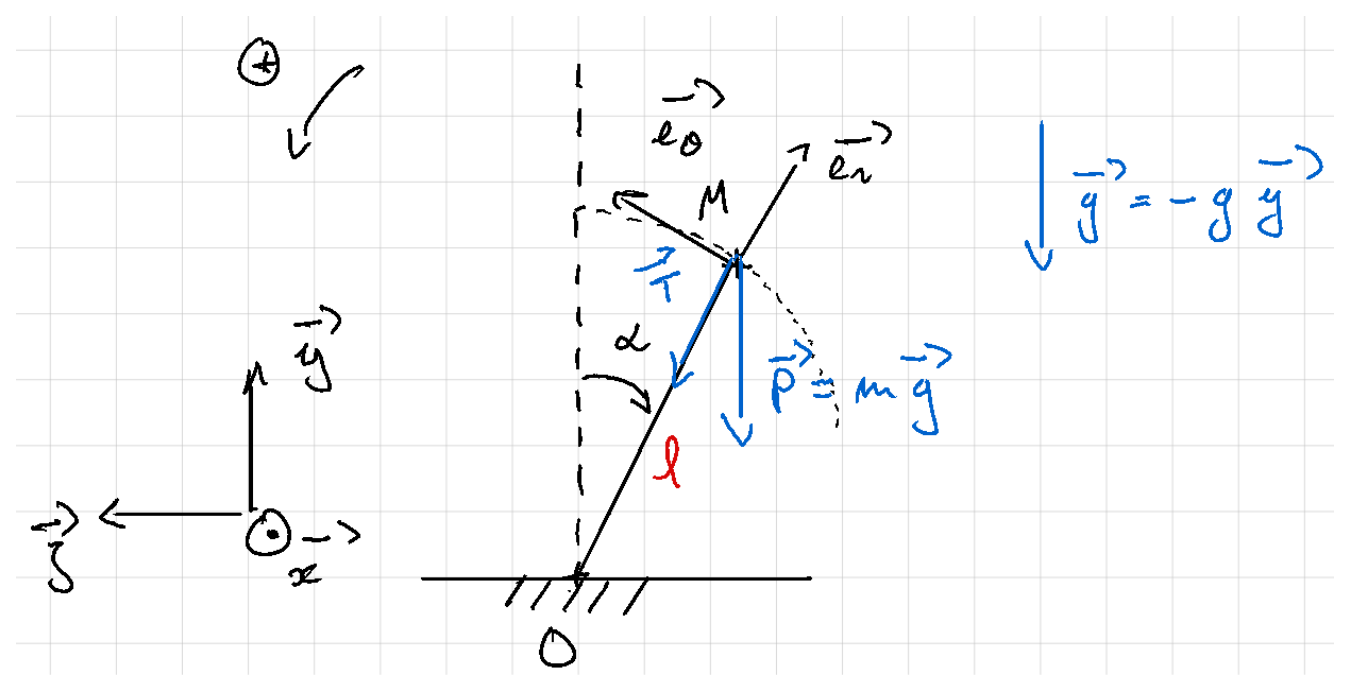
\includegraphics[scale=0.25]{images/schema_pendule_inverse_fixe.png}
                        \caption{Schéma du pendule inversé simple fixe en $O$}
                        \label{fig_pendule_inverse_fixe}
                \end{figure}

                \begin{figure}[h!]
                        \centering
                        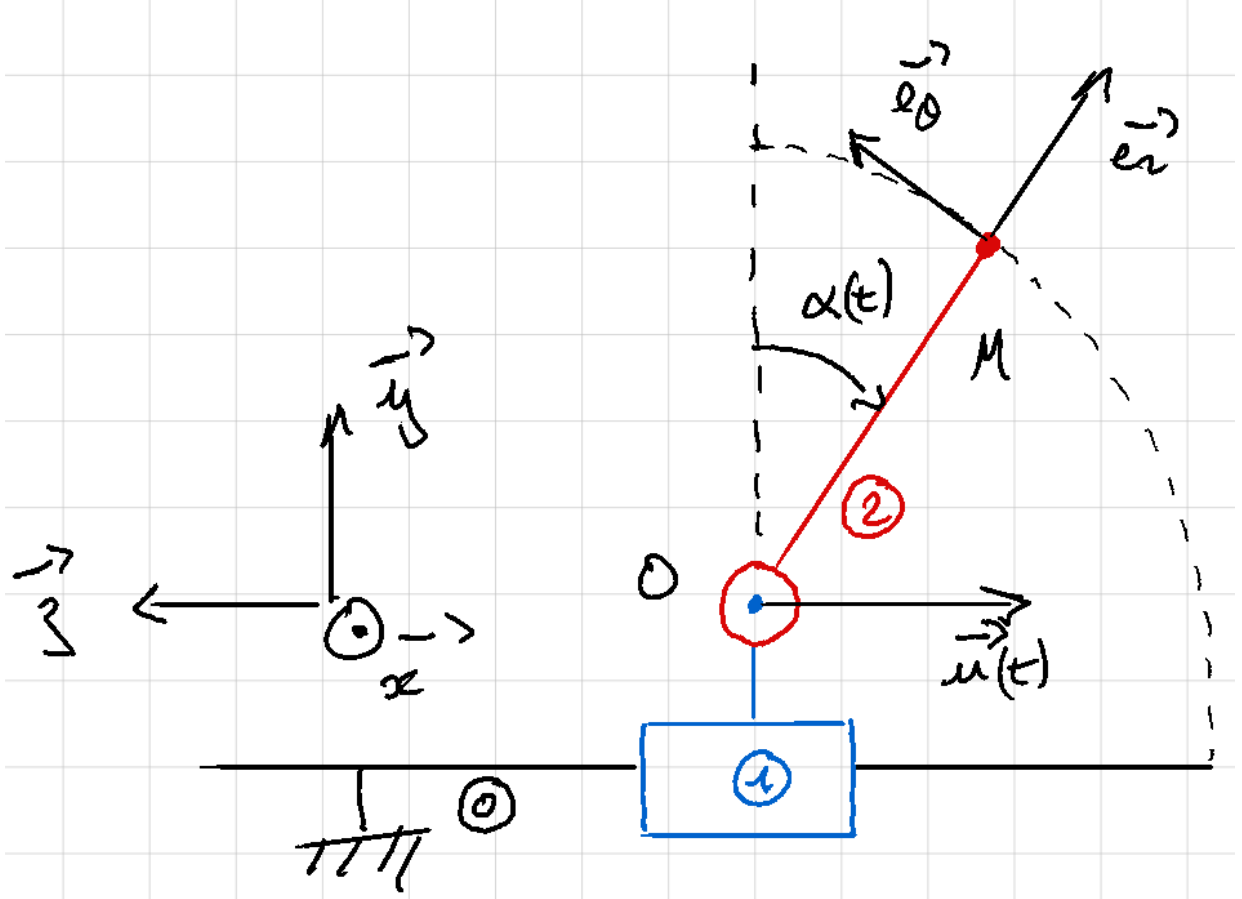
\includegraphics[scale=0.2]{images/schema_pendule_inverse_controle.png}
                        \caption{Schéma du pendule inversé contrôlé en accélération suivant l'axe $(O,\vec{z})$}
                        \label{fig_pendule_inverse_controle}
                \end{figure}

                Avec :
                \begin{itemize}
                        \item $\overrightarrow{OM} = l \vec{e}_r$
                        \item $\alpha$ angle entre la normale du support et le pendule en $rad$ 
                        \item $l$ la longueur du pensule en $m$
                        \item $u(t)$ en $m.s^{-1}$
                \end{itemize}

        \section{Modèle dynamique du système}

                \subsection{Equation d'état du système}

                        Nous allons dans cette pratie mettre en équations le comportement dynamique du \textit{Robot Lego Segway}
                        en exploitant dans un premier temps le modèle du pendule simple inversé non contrôlé, puis celui
                        du pendule inversé contrôlé et enfin un modèle plus complet se rapprochant du fonctionnement du système réel.

                        \subsubsection{Modèle du pendule inversé}

                                On considère le modèle du pendule simple inversé, schématisé par la figure \ref{fig_pendule_inverse_fixe}.
                                Notre démarche est la suivante : \\

                                \underline{\textit{Système isolé :}} \{Point $M$ de masse $m$\} \\

                                \underline{\textit{Référentiel :}} Référentiel lié au repère $\mathcal{R} = (O,\vec{x}, \vec{y}, \vec{z})$ supposé galiléen \\

                                \underline{\textit{Bilan des forces extérieures :}} \\
                                
                                \begin{itemize}
                                        \item $\overrightarrow{T}=T\vec{e}_r$ avec $T$ en $N$
                                        \item $\overrightarrow{P}=mg\vec{y}$ avec $m$ en $kg$ et $g$ la constante gravitationnelle terrestre en $m.s^{-2}$
                                \end{itemize}
                                Le principe fondamental de la dynamique projeté suivant la direction de $\vec{e}_\theta$ nous donne l'équation d'état suivante : 
                                \begin{equation}
                                        \ddot \alpha (t) = \frac{g}{l} \sin (\alpha (t))
                                        \label{eq1}
                                \end{equation}

                                Ou encore en posant $x=(\alpha, \dot \alpha)$ et $f : \vspace{15pt} \left\{
                                \begin{array}{rcl}
                                        \mathbb{R}^2 \times \mathbb{R} & \mapsto & \mathbb{R}^2 \\
                                        (x,u) & \to & f(x,u) = \begin{bmatrix} \dot \alpha (t)\\ \frac{g}{l} \sin (\alpha (t)) \end{bmatrix}
                                \end{array} \right.$ :

                                \begin{equation}
                                        \dot x = f(t,x(t))
                                        \label{eq2}
                                \end{equation}
                                \vspace{5pt}

                                On considère à présent le modèle du pendule inversé contrôlé en accélération suivant l'axe $(O,\vec{z})$
                                tel qu'il est schématisé sur la figure \ref{fig_pendule_inverse_controle}.
                                On explicitera plus en détail dans la partie commande du système (partie \ref{commande_du_systeme}) ce que signifie
                                exactement le terme contrôlé. Ici, il s'agit uniquement de mettre en équation le système modélisé par le schéma cinématique.
                                Notre démarche est la suivante : \\

                                \underline{\textit{Système isolé :}} $(\Sigma) = \{$Point $M$ de masse $m\}$ où seul la masse $m$ du point $M$ est considérée\\

                                \underline{\textit{Référentiel :}} Référentiel lié au repère $\mathcal{R} = (O',\vec{x}, \vec{y}, \vec{z})$ supposé galiléen
                                où $O'$ est un point fixe du batit (0). \\

                                \underline{\textit{Inventaire des actions mécaniques extérieures :}} \\

                                \begin{itemize}
                                        \item $\{\mathcal{T}_{\overrightarrow{P} \to (\Sigma)} \} = \left\{ 
                                        \begin{array}{cc}
                                                -mg\vec{y} \\
                                                \vec{0}
                                        \end{array} \right\}_{M,\mathcal{R}}
                                        = \left\{
                                        \begin{array}{cc}
                                                -mg\vec{y} \\
                                                \sin (\alpha)mgl\vec{x}
                                        \end{array} \right\}_{M,\mathcal{R}}$
                                \end{itemize}

                                On montre à l'aide d'un théorème du moment statique appliqué en $O$ à \{(1)\} que $L_{01}=0$.
                                On obtient par la suite, en appliquant le théorème du moment dynamique en $O$ à ($\Sigma$) et projeté
                                suivant la direction de $\vec{x}$ l'équation suivante :
                                \begin{equation}
                                        \ddot \alpha = \frac{g}{l}\sin (\alpha) - \frac{\cos (\alpha) \dot u}{l}
                                        \label{eq3}
                                \end{equation}

                                NB : On a supposé que l'accélération $\dot \alpha \sin(\alpha)u$ était négligeable devant l'accélération du solide
                                et devant son accélération angulaire.


                                On peut également vectoriser l'équation (\ref{eq3}) en posant $x=(\alpha, \dot \alpha)$ et : $$h : \vspace{15pt} \left\{
                                \begin{array}{rcl}
                                        \mathbb{R}^2 \times \mathbb{R} & \mapsto & \mathbb{R}^2 \\
                                        (x,a(t)) & \to & \begin{bmatrix} \dot \alpha \\ \frac{g}{l} \sin (\alpha) - \frac{\cos (\alpha) \dot u}{l}\end{bmatrix}
                                \end{array} \right.$$
                                où $a$ : $t \mapsto a(t) = \dot u(t)$.

                                On peut alors de nouveau écrire le problème sous la forme :
                                \begin{equation}
                                        \dot x = f(t,x(t),a(t))
                                        \label{eq4}
                                \end{equation}

                                On remarque les équations (\ref{eq3}) et (\ref{eq4}) sont très proches respectivement
                                des équations (\ref{eq1}) et (\ref{eq2}) mais avec un terme que l'on pourra qualifier de terme
                                de contrôle et que l'on explicitera dans les parties suivantes.


                        \subsubsection{Modèle du robot Lego}

                                En ce qui concerne la mise en équations du comportement du modèle plus complet du \textit{Robot Lego Segway}
                                schématisé par le schéma cinématique de la figure \ref{fig_robot_lego} 
                                on obtient, par une méthode analogue à celle ci-dessus et en employant les principes fondamentaux de la dynamique,
                                le système d'équations différentielles couplées suivant : 
                                
                                $$
                                \begin{cases}
                                        \ddot \theta = \frac{C_4 C_3 - C_2 C_5 + C_4 C_{\theta} (U(t), \dot \theta (t), \dot \psi (t)) - C_2 C_{\psi} (U(t), \dot \theta (t), \dot \psi (t))}{C_4 C_1 - C_2^2} \\
                                        \ddot \psi = \frac{C_{\psi} (U(t), \dot \theta (t), \dot \psi (t)) - C_2 \ddot \theta - C_5}{C_4}
                                \end{cases}
                                $$

                                Voir la partie \ref{equations_robot_lego} en Annexe pour les unités et le détails des paramètres. \\


                \subsection{Stabilité du système non contrôlé}

                        On rappelle que les équations qui régissent le pendule inversé contrôlé sont les suivantes :
                        $$
                        (S)
                        \begin{cases}
                            \dot x_1(t) = x_2(t) \\
                            \dot x_2(t) = \frac{g}{l} \sin (s_1(t)) - \frac{\cos (x_1(t))u(t)}{l} \\
                            x_1(0) = x_{0,1} = \alpha _0 \\
                            x_2(0) = x_{0,2} = \dot \alpha _0
                        \end{cases}
                        $$

                        avec :

                        \begin{itemize}
                                \item $g=9.81$
                                \item $l=10$
                                \item $x_e=(0,0)$
                                \item $u_e = 0$
                                \item $u(t) = u_e + K(x(t) - x_e)$
                                \item $K = \begin{bmatrix} k_1 & k_2 \end{bmatrix}$
                        \end{itemize}

                        Soit $(\Sigma) 
                        \begin{cases} 
                                \dot x_1(t) = x_2(t) \\
                                \dot x_2(t) = \frac{g}{l} \sin (x_1(t)) - \frac{\cos (x_1(t))}{l} u(t)
                        \end{cases}$.

                        \vspace{10pt}

                        $(\Sigma)$ s'écrit $\dot x(t) = f(x(t), u(t))$ où $f : \left\{
                        \begin{array}{rcl}
                            \mathbb{R}^2 \times \mathbb{R} & \mapsto & \mathbb{R}^2 \\
                            (x,u) & \to & f(x,u) = \begin{bmatrix} x_2 \\ \frac{g}{l} \sin x_1 - \frac{\cos x_1}{l} u \end{bmatrix}
                        \end{array} \right.$

                        \vspace{10pt}

                        On veut déterminer la stabilité, stabilité asymptotique ou instabilité de l'origine.
                        On considère alors $\forall t \in \mathbb{R}, u(t) = 0$ et $\dot x(t) = f(x(t), 0) \overset{def}{=} g(x(t))$ c'est-à-dire $f(x,0)$. \\
                        On a $g(x_e)=0$ donc $x_e$ est bien un point d'équilibre.

                        On calcule la jacobienne de $g$ :
                        $$
                        g'(x) = 
                        \begin{bmatrix}
                                \frac{\partial f_1(x,0)}{\partial x_1}(x) & \frac{\partial f_1(x,0)}{\partial x_2}(x) \\
                                \frac{\partial f_2(x,0)}{\partial x_1}(x) & \frac{\partial f_2(x,0)}{\partial x_2}(x)
                        \end{bmatrix}
                        =
                        \begin{bmatrix}
                                0 & 1 \\
                                \frac{g}{l} \cos x_1 & 0
                        \end{bmatrix}
                        \Longrightarrow
                        g'(x_e) = 
                        \begin{bmatrix}
                                0 & 1 \\
                                \frac{g}{l} & 0
                        \end{bmatrix}
                        $$

                        On a donc 
                        $
                        \begin{cases} 
                            \tr g'(x_e) = 0 \\ 
                            \det g'(x_e) = - \frac{g}{l} < 0
                        \end{cases}
                        \Longrightarrow 
                        \lambda_{\pm}  = \pm \sqrt{\frac{g}{l}}
                        $
                        donc il existe une valeur propre à partie réelle $> 0$ ce qui implique que $x_e$ est instable. \\

        \section{Commande du système}
        \label{commande_du_systeme}

                \subsection{Stabilisation par retour d'état autour d'un point d'équilibre}

                        La stabilisation par retour d'état consiste à boucler un système en boucle ouverte afin de prendre en compte
                        l'état de sortie du système à l'instant $t$ pour corriger ce dernier en fonction de la consigne donnée à l'instant $t+1$.
                        L'acquisition de l'état de sortie su système se fait en réalité à l'aide de capteur. Tout ceci peut être schématisé par les
                        figures \ref{fig_systeme_boucle_ouverte} et \ref{fig_systeme_boucle_fermee}. \\
                        
                        \begin{figure}[h!]
                                \centering
                                \begin{subfigure}[b]{0.45\textwidth}
                                        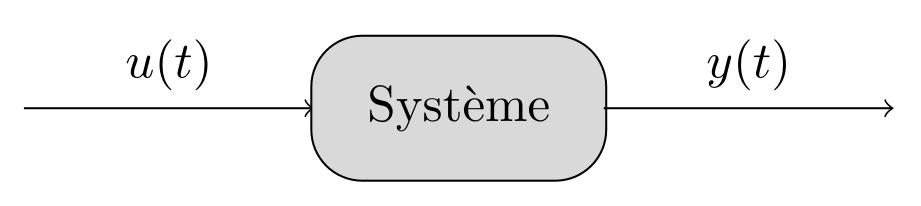
\includegraphics[width=\textwidth]{images/schema_systeme_boucle_ouverte.png}
                                        \caption{Schéma fonctionnel d'un système en boucle ouverte}
                                        \label{fig_systeme_boucle_ouverte}
                                \end{subfigure}
                                \hspace{30pt}
                                \begin{subfigure}[b]{0.45\textwidth}
                                        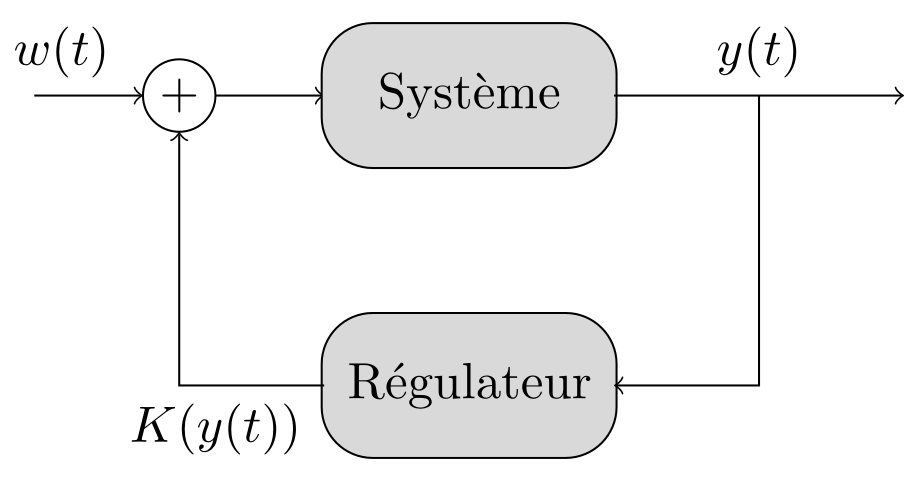
\includegraphics[width=\textwidth]{images/schema_systeme_boucle_fermee.png}
                                        \caption{Schéma fonctionnel d'un systeme en boucle fermée par retour de sortie}
                                        \label{fig_systeme_boucle_fermee}
                                \end{subfigure}
                                \caption{Schémas de systèmes en boucle ouverte et fermée}
                                \label{fig_systeme_boucle}
                        \end{figure}


                        La correction ou le contrôle se traduit par l'expression $u(t) = w(t) + K(y(t))$ avec $K$ : $\mathbb{R}^p \to \mathbb{R}^n$
                        où $p$ est le nombre de pramaètres à la sortie et $n$ le nombre de paramètres en entrée.
                        En particulier, le terme \textit{par retour d'état} vient du fait que $y(t) = x(t)$. On a donc $K$ : $\mathbb{R}^n \to \mathbb{R}^n$.


                        La stabilisation par retour d'état autour d'un point d'équilibre signifie simplement que l'on va vouloir trouver la bonne application
                        $K$ qui permet de stabiliser asymptotiquement le système autour d'un point d'équilibre noté $x_e$ (point tel que pour $f$, la fonction
                        caractérisant le comportement dynamique du système, on ait : $f(x_e) = 0$).


                        On cherchera par la suite à déterminer la valeur de $w(t)$ est noté $u_e$ et le couple $(x_e,u_e)$ correspond au point de fonctionnement
                        du système contrôlé, c'est-à-dire le point qui assure la stabilisation du système autour de sa position d'équilibre $x_e$ en régime
                        stationnaire (point tel que pour $f$ on ait $f(x_e,u_e)$ = 0).


                        \subsubsection{Stabilisation du pendule inversé}
                        \label{stabilisation_pendule_inverse}

                        On cherche maintenant des conditions sur $K$ pour que le contrôle par retour d'état
                        $u(t) = u_e + K(x(t)-x_e)$ stabilise asymptotiquement le système à l'origine.
                        On note $g(x(t)) \overset{def}{=} \dot x(t) = f(x(t), u_e + K(x(t)-x_e))$.
                        On a donc :
                        $$
                        g(x) = 
                        \begin{bmatrix}
                                x_2 \\
                                \frac{g}{l} \sin x_1 - \frac{\cos x_1}{l} (u_e+k_1x_1+k_2x_2)
                        \end{bmatrix}
                        $$

                        Donc
                        $$
                        g'(x) = 
                        \begin{bmatrix}
                                0 & 1 \\
                                -\frac{\cos x_1}{l} k_2 & \frac{g}{l}\cos x_1 + \frac{\sin x_1}{l}(u_e+k_1x_1+k_2x_2) - \frac{\cos x_1}{l}k_1
                        \end{bmatrix}
                        $$
                        $$
                        \Longrightarrow
                        g'(x_e) =
                        \begin{bmatrix}
                                0 & 1 \\
                                \frac{g-k_1}{l} & -\frac{k_2}{l}
                        \end{bmatrix}
                        $$

                        Donc on obtient :
                        $$
                        \begin{cases}
                                \tr g'(x_e) = -\frac{k_2}{l} < 0 \\
                                \det g'(x_e) = \frac{k_1-g}{l} > 0
                        \end{cases}
                        \Longleftrightarrow
                        \begin{cases}
                                k_1 > g \\
                                k_2 > 0
                        \end{cases}
                        $$
                        \vspace{10pt}

                        Ainsi, en respectant ces deux conditions, on obtient avec $x_0=(\pi/20,0)$ et $K=(30,10)$ 
                        les courbes resprésentées sur la figure \ref{fig3.1}.
                        \begin{figure}[h!]
                            \centering
                            \begin{subfigure}[b]{0.45\textwidth}
                                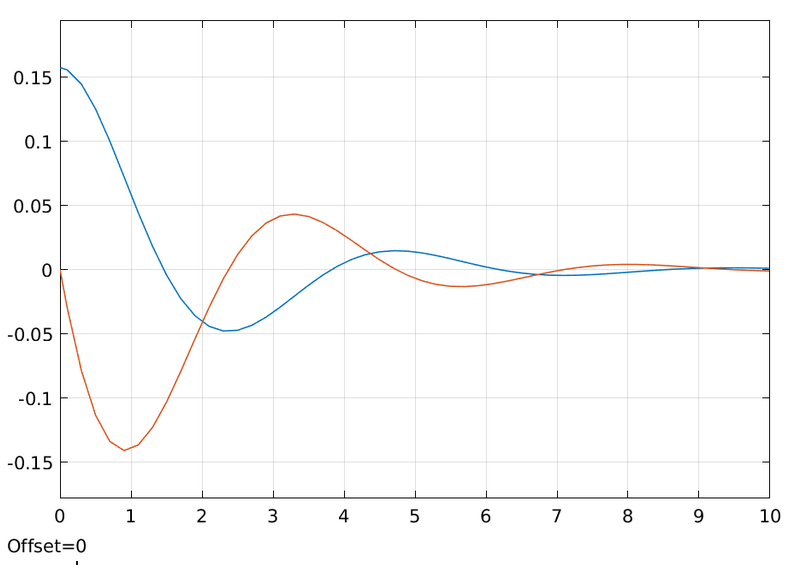
\includegraphics[width=\textwidth]{images/courbe_cas_1_1_TP02.png}
                                \caption{Etat}
                                \label{fig3.1.1}
                            \end{subfigure}
                            \hspace{30pt}
                            \begin{subfigure}[b]{0.45\textwidth}
                                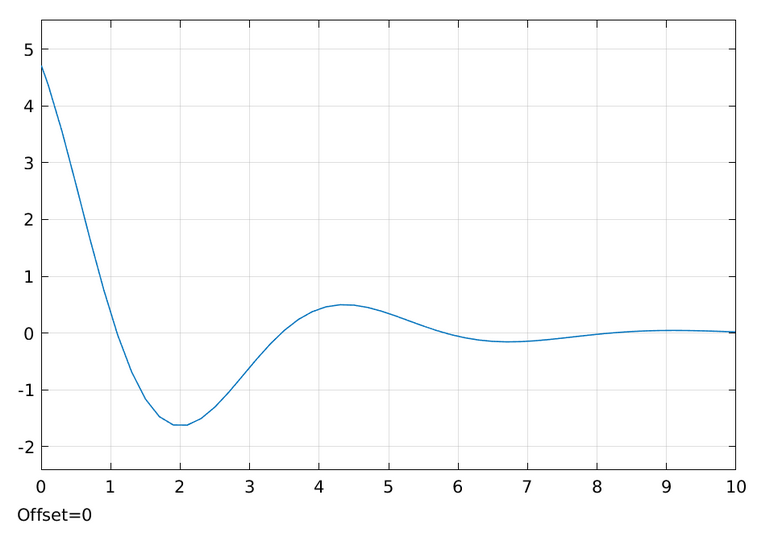
\includegraphics[width=\textwidth]{images/controle_cas_1_1_TP02.png}
                                \caption{Contrôle}
                                \label{fig3.1.2}
                            \end{subfigure}
                            \caption{Cas 1.1 avec $x_0=(\pi/20, 0)$ et $K=(30,10)$}
                            \label{fig3.1}
                        \end{figure} \\
                        On remarque que le système se stabilise asymptotiquement vers son point d'équilibre $x_e=(0,0)$.
                        En ce qui concerne la courbe du contrôle en accélération, elle a la même allure que la courbe de l'angle $\alpha$
                        du pendule (courbe bleu sur la figure \ref{fig3.1.1}), ce qui fait sens. 
                        En effet, lorsque l'on perturbe l'équilibre du pendule en lui imposant une position initiale avec un angle strictement positif,
                        la base du pendule va accélérer dans le sens positif du déplacement.
                        De même, le support va accélérer dans le sens des $z$ décroissants lorsque l'angle sera négatif.
                        La base du pendule accélère donc dans le même sens que la perturbation pour la compenser. \\


                        En pratique, on n'a accès qu'à $\dot \alpha$.
                        On ajoute alors en plus du contrôleur, un capteur et un prédicteur pour reconstruire $\alpha$.

                        \begin{table}[h!]
                                \centering
                                \begin{tabular}{|c||c|c|c|c|c|} \hline
                                        \textbf{Cas} & \textbf{$x_0$} & \textbf{$t_f$} & \textbf{$K$} & \textbf{Pas} & \textbf{Intégrateur} \\ \hline
                                        Cas 2.1 & $(\pi/20,0)$ & 100 & (10,1) & par défaut & ode45 \\ \hline
                                        Cas 2.2 & $(\pi/20,0)$ & 100 & (10,1) & 0.001 & ode45 \\ \hline
                                        Cas 2.3 & $(\pi/20,0)$ & 100 & (10,1) & 5 & Euler, ode1 \\ \hline
                                \end{tabular}
                                \label{table2}
                                \caption{Paramètres de tests pour le retour d'état du pendule inversé avec capteur et prédicteur}
                        \end{table}

                        On obtient alors les résulats présents sur les figures \ref{fig3.2} et \ref{fig3.3} et \ref{fig3.4}.
                        \begin{figure}[h!]
                                \centering
                                \begin{subfigure}[b]{0.45\textwidth}
                                        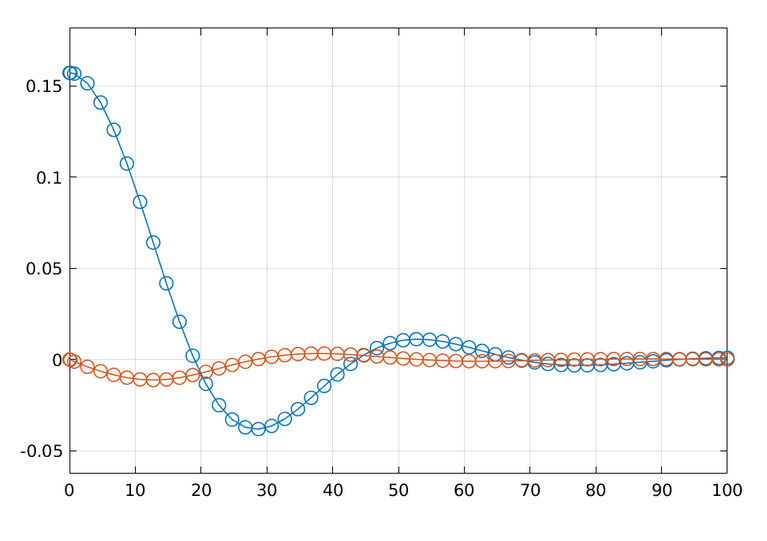
\includegraphics[width=\textwidth]{images/courbe_cas_2_1_TP02.png}
                                        \caption{Etat}
                                        \label{fig3.2.1}
                                \end{subfigure}
                                \hspace{30pt}
                                \begin{subfigure}[b]{0.45\textwidth}
                                        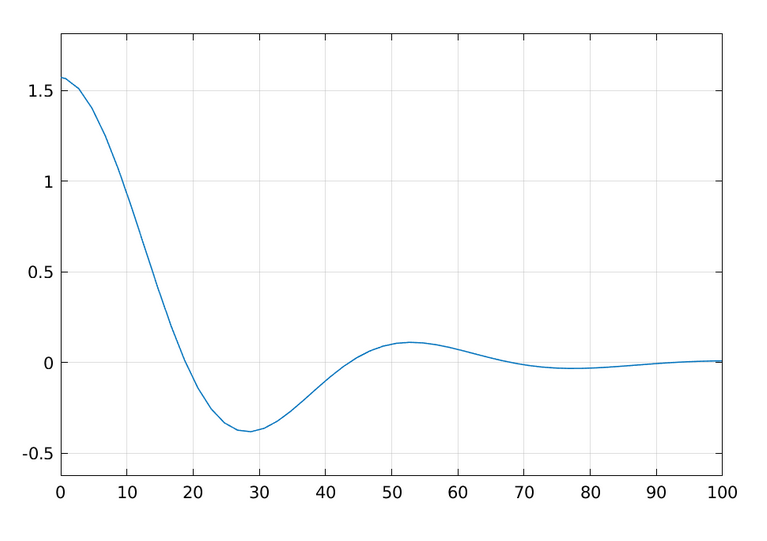
\includegraphics[width=\textwidth]{images/controle_cas_2_1_TP02.png}
                                        \caption{Contrôle}
                                        \label{fig3.2.2}
                                \end{subfigure}
                                \caption{Cas 2.1 avec $x_0=(\pi/20, 0)$, $K=(10,1)$ et un pas d'intégration par défaut}
                                \label{fig3.2}
                        \end{figure}

                        \begin{figure}[h!]
                                \centering
                                \begin{subfigure}[b]{0.45\textwidth}
                                        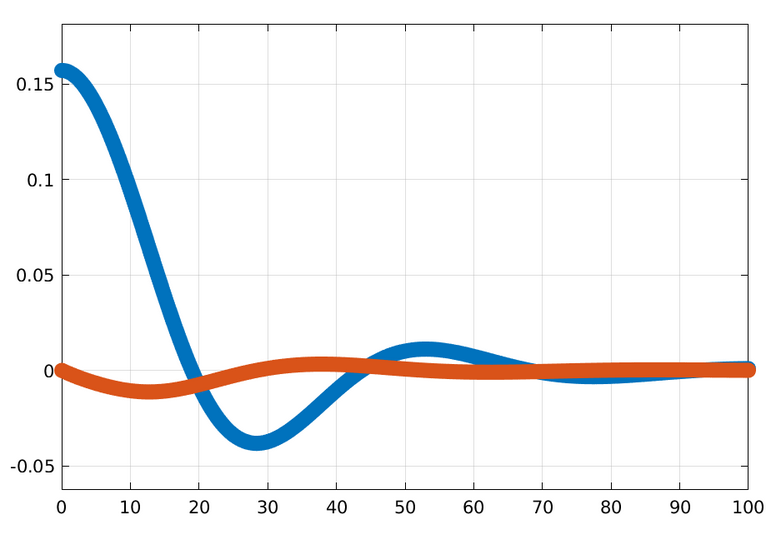
\includegraphics[width=\textwidth]{images/courbe_cas_2_2_TP02.png}
                                        \caption{Etat}
                                        \label{fig3.3.1}
                                \end{subfigure}
                                \hspace{30pt}
                                \begin{subfigure}[b]{0.45\textwidth}
                                        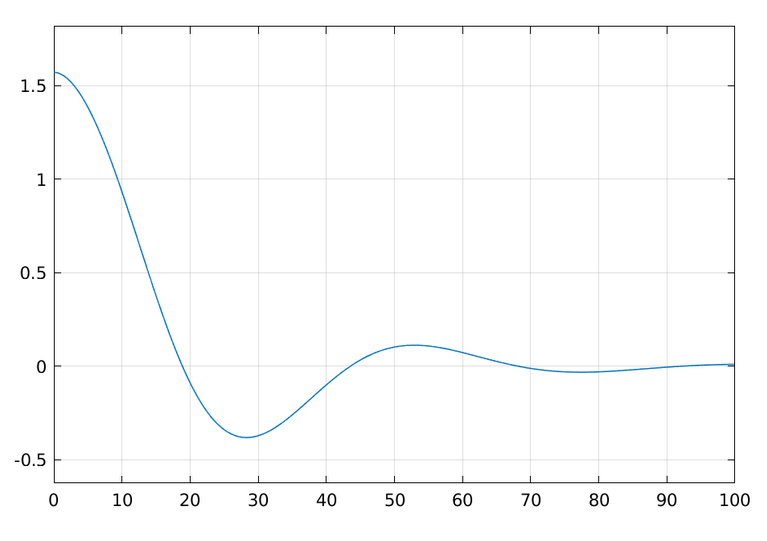
\includegraphics[width=\textwidth]{images/controle_cas_2_2_TP02.png}
                                        \caption{Contrôle}
                                        \label{fig3.3.2}
                                \end{subfigure}
                                \caption{Cas 2.2 avec $x_0=(\pi/20, 0)$, $K=(10,1)$ et un pas d'intégration de 0.001}
                                \label{fig3.3}
                        \end{figure}

                        \begin{figure}[h!]
                                \centering
                                \begin{subfigure}[b]{0.45\textwidth}
                                        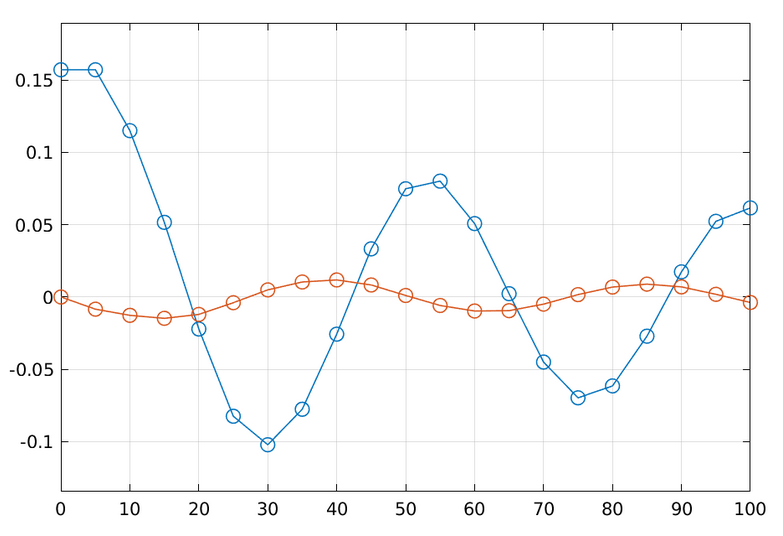
\includegraphics[width=\textwidth]{images/courbe_cas_2_3_TP02.png}
                                        \caption{Etat}
                                        \label{fig3.4.1}
                                \end{subfigure}
                                \hspace{30pt}
                                \begin{subfigure}[b]{0.45\textwidth}
                                        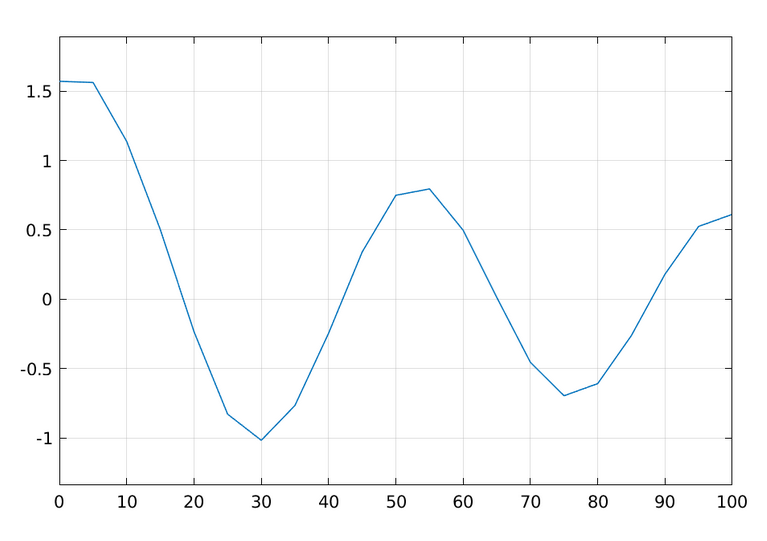
\includegraphics[width=\textwidth]{images/controle_cas_2_3_TP02.png}
                                        \caption{Contrôle}
                                        \label{fig3.4.2}
                                \end{subfigure}
                                \caption{Cas 2.3 avec $x_0=(\pi/20, 0)$, $K=(10,1)$ et un pas d'intégration de 5}
                                \label{fig3.4}
                        \end{figure}


                        On remarque que lorsqu'on augmente le pas d'intégration, on ne peut plus considérer le signal de sortie comme un signal continu.
                        De plus, on remarque également que cela impacte la stabilité du système puisqu'on observe sur la figure  
                        que les oscillations sont plus importantes. En effet, on relève un premier dépassement en pourcentages pour les courbes des
                        figures \ref{fig3.2.1} et \ref{fig3.3.1} $D_{1\%} \simeq 25\%$ contre $D_{1\%} \simeq 64\%$
                        pour la courbe de la figure \ref{fig3.4.1}.
                        On remarque aussi que le système met plus de temps à converger asymptotiquement vers son point d'équilibre.
                        Effectivement, on relève un temps de réponse à 5\% pour les courbes des figures \ref{fig3.2.1} et \ref{fig3.3.1}
                        $t_{5\%} \simeq 55$s contre $t_{5\%} > 100$s pour la courbe de la figure \ref{fig3.4.1}.
                        On remarque aussi que la courbe du contrôle en fonction du temps, qui est un contrôle en accélération,
                        ne peut plus être considérée comme un signal continu si le pas d'intégration devient trop grand. 
                    

                \subsubsection{Stabilisation du robot Lego}

                        Après avoir étudié le modèle du pendule inversé, le but de cette partie est d'étudier le modèle du robot Lego pendule inversé.
                        On se propose alors de construire un modèle \textsc{Simulink} comportant un bloc avec l'équation d'état du système et un contrôleur par retour d'état.
                        L'objectif est alors de calculer les coefficients de la matrice $K$.
                        Pour ce faire, on linéarise le système d'équations différentielles du modèle du robot Lego
                        pour se ramener à une forme $\dot x(t) = (A+BK)x(t)$ et on détermine l'expression de la matrice $A+BK$.
                        Par la suite on détermine la valeur des coefficients de $K$ à partir des valeurs des pôles du système que l'on se fixe
                        (les valeurs des pôles sont fixées tel que leur partie réelle soit strictement négative ou que une seule seulement soit nulle).

                        \begin{table}[h!]
                                \centering
                                \begin{tabular}{|c||c|c|c|c|} \hline
                                        \textbf{Cas} & \textbf{$x_0$} & \textbf{$t_f$} & \textbf{$K$} & \textbf{Intégrateur} \\ \hline
                                        Cas 1.1 & $(0,0,0,0)$ & 2 & $K$ & ode45 \\ \hline
                                        Cas 1.2 & $(0,\pi/5,0,0)$ & 5 & $K$ & ode45 \\ \hline
                                        Cas 1.3 & $(0,\pi/10,0,0)$ & 5 & $K$ & ode45 \\ \hline
                                \end{tabular}
                                \label{table3}
                                \caption{Paramètres de tests pour le retour d'état du robot Lego pendule inversé sans capteur ni prédicteur}
                        \end{table}

                        Après avoir simulé ce modèle, on obtient les résultats présents dans les figures \ref{fig3.5}, \ref{fig3.6} et \ref{fig3.7}.
                        \begin{figure}[h!]
                                \centering
                                \begin{subfigure}[b]{0.45\textwidth}
                                        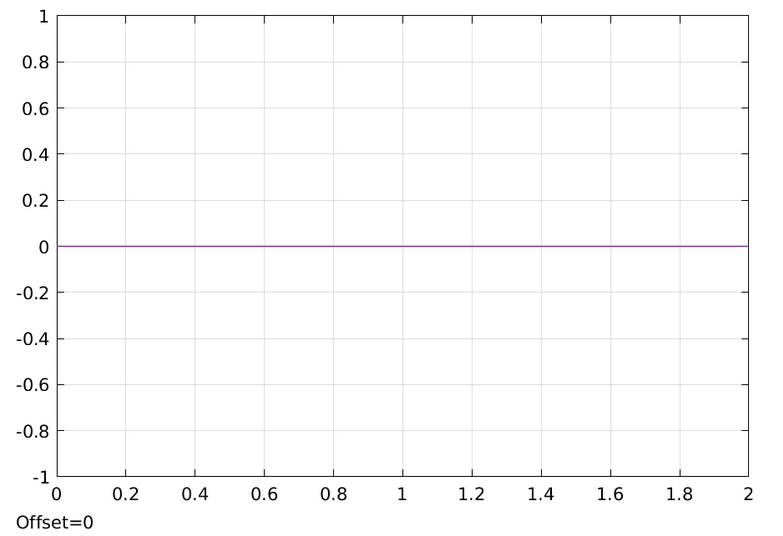
\includegraphics[width=\textwidth]{images/courbe_cas_1_1_TP03.png}
                                        \caption{Etat}
                                        \label{fig3.5.1}
                                \end{subfigure}
                                \hspace{30pt}
                                \begin{subfigure}[b]{0.45\textwidth}
                                        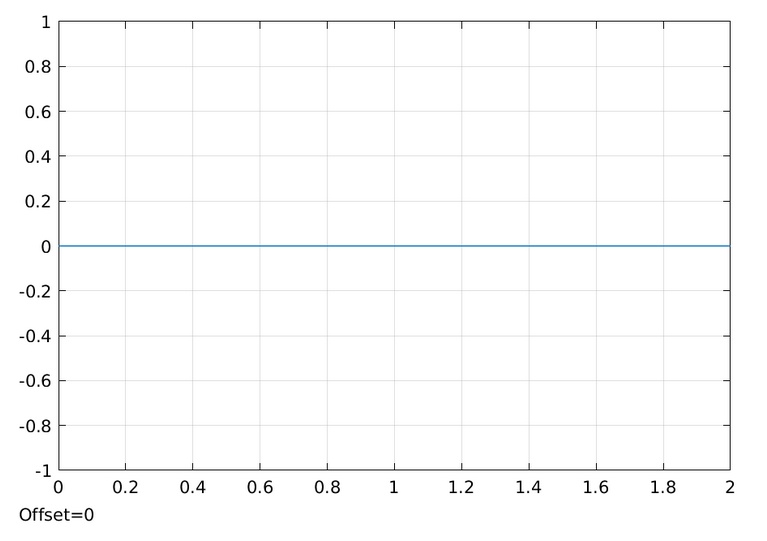
\includegraphics[width=\textwidth]{images/controle_cas_1_1_TP03.png}
                                        \caption{Contrôle}
                                        \label{fig3.5.2}
                                \end{subfigure}
                                \caption{Cas 1.1 avec $x_0=(0,0,0,0)$}
                                \label{fig3.5}
                        \end{figure}

                        \begin{figure}[h!]
                                \centering
                                \begin{subfigure}[b]{0.45\textwidth}
                                        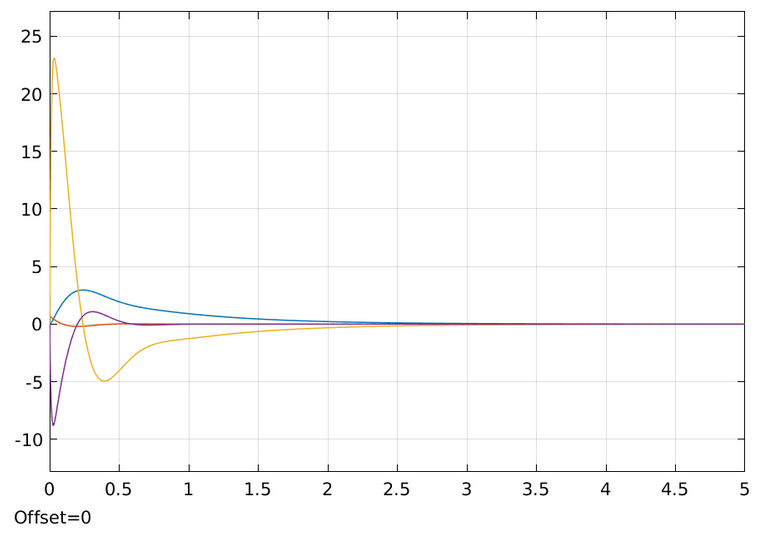
\includegraphics[width=\textwidth]{images/courbe_cas_1_2_TP03.png}
                                        \caption{Etat}
                                        \label{fig3.6.1}
                                \end{subfigure}
                                \hspace{30pt}
                                \begin{subfigure}[b]{0.45\textwidth}
                                        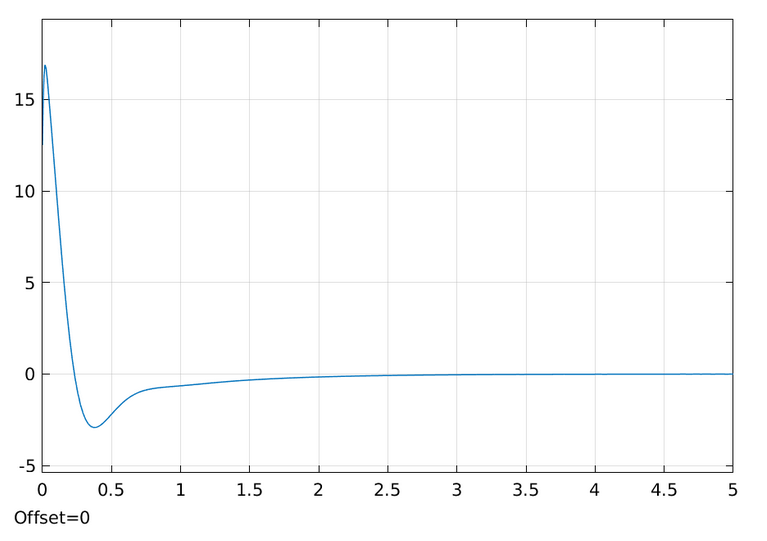
\includegraphics[width=\textwidth]{images/controle_cas_1_2_TP03.png}
                                        \caption{Contrôle}
                                        \label{fig3.6.2}
                                \end{subfigure}
                                \caption{Cas 1.2 avec $x_0=(0,\pi/5,0,0)$}
                                \label{fig3.6}
                        \end{figure}
                        \newpage


                        \begin{figure}[h!]
                                \centering
                                \begin{subfigure}[b]{0.45\textwidth}
                                        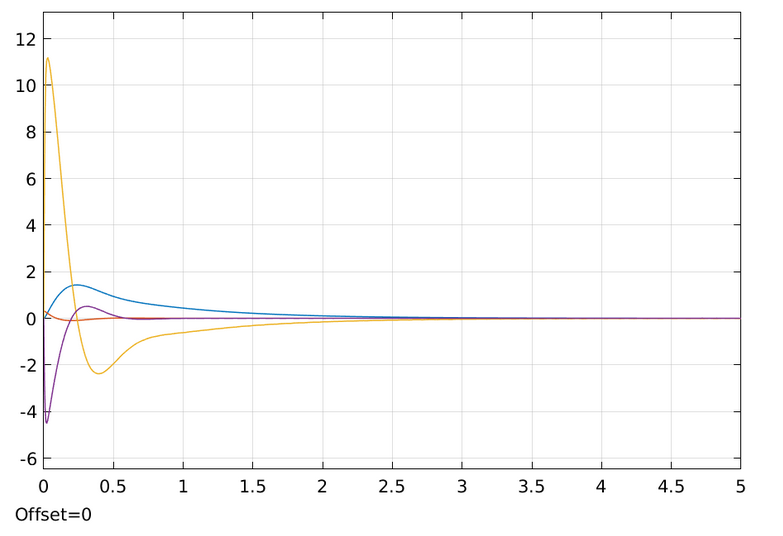
\includegraphics[width=\textwidth]{images/courbe_cas_1_3_TP03.png}
                                        \caption{Etat}
                                        \label{fig3.7.1}
                                \end{subfigure}
                                \hspace{30pt}
                                \begin{subfigure}[b]{0.45\textwidth}
                                        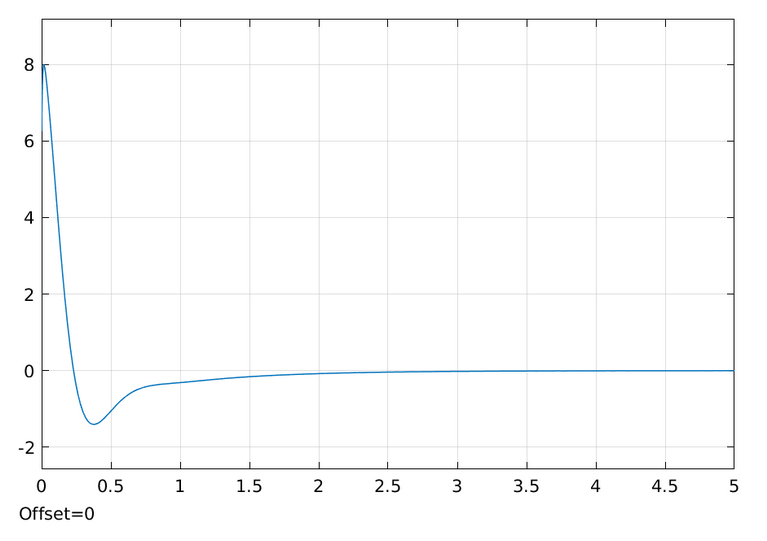
\includegraphics[width=\textwidth]{images/controle_cas_1_3_TP03.png}
                                        \caption{Contrôle}
                                        \label{fig3.7.2}
                                \end{subfigure}
                                \caption{Cas 1.3 avec $x_0=(0,\pi/10,0,0)$}
                                \label{fig3.7}
                        \end{figure}

                        On remarque que lorsque le système est en position initiale au point d'équilibre $x_e=(0,0,0,0)$, il y reste
                        (figure \ref{fig3.5.1} : courbe jaune angle $\psi$ en $deg$). 
                        Ensuite, lorsque la position initiale n'est pas au point d'équilibre, le système converge toujours asymptotiquement vers
                        sa position d'équilibre en un temps relativement rapide (cas 1.2 avec $t_{5\%} \simeq 1.3s$ et cas 1.3 avec $t_{5\%} \simeq 1.2s$)
                        (figures \ref{fig3.6.1} et \ref{fig3.7.1} : courbe jaune). \\

                        En ce qui concerne le paramètre $\theta$, qui correspond comme illustré sur la figure \ref{fig_robot_lego},
                        à l'angle $\psi + \theta_m$, on remarque sur les figures \ref{fig3.6.1} et \ref{fig3.7.1} qu'il s'éloigne de la
                        position angulaire $0^{°}$ pour y converger de nouveau une fois que le robot se stabilise. Ce qui signifie que $\theta$ croît puis décroît.
                        Cela se traduit physiquement par le fait que la stabilisation du robot se fait en deux phases : une première où il avance en accélérant
                        et une deuxième où il recule en accélérant dans la direction opposée pour se retrouver à son point de départ mais avec un angle
                        $\psi$ de $0^{°}$ (courbes bleues sur les figures \ref{fig3.6.1} et \ref{fig3.7.1}). \\

                        Pour les deux paramètres restants qui sont $\dot \theta$ (courbe rouge) et $\dot \psi$ (courbe violette), on remarque que pour les cas 2.2 et 2.3, 
                        seul la valeur de $\dot \psi$ varie significativement. \\

                        Pour ce qui est de la valeur de $\dot \theta$, on remarque dans les deux cas qu'elle est presque tout le temps nulle sauf initialement où
                        le robot est écarté de sa position d'équilibre et converge vers cette dernière.
                        Or comme $\dot \theta = \dot \psi + \dot \theta_m$, cela peut s'interpréter par le fait que la vitesse angulaire des deux angles se compensent,
                        ce qui est probablement lié au contrôle en accélération qui a pour but de s'opposer à la perturbation en position angulaire du système. \\

                        Pour ce qui est de la valeur de $\dot \psi$, on remarque dans tous les cas que son signe est opposé à la position angulaire $\psi$ du robot.
                        Cela traduit bien le fait que l'évolution de la position angulaire du robot en fonction du temps est amortie et converge vers sa position d'équilibre.
                        Donc le contrôle est bien actif. \\

                        En ce qui concerne l'évolution de la courbe du contrôle en accélération, les remarques et l'interprétation physique sont les mêmes que pour
                        la partie \ref{stabilisation_pendule_inverse} avec la figure \ref{fig3.3}. \\

                        En pratique, un gyroscope mesure la vitesse de changement d'angle du corps du robot, que l'on note $\dot \psi (t)$
                        et un capteur mesure l'angle que l'on note $\theta (t)$.
                        On implémente alors un sous-système prédicteur qui permet de restituer les informations manquantes, à savoir
                        $\psi (t)$ et $\dot \theta (t)$.


                        \begin{table}[h!]
                                \centering
                                \begin{tabular}{|c||c|c|c|c|} \hline
                                        \textbf{Cas} & \textbf{$x_0$} & \textbf{$t_f$} & \textbf{$K$} & \textbf{Intégrateur} \\ \hline
                                        Cas 2.1 & $(0,0,0,0)$ & 2 & $K$ & ode45 \\ \hline
                                        Cas 2.2 & $(0,\pi/5,0,0)$ & 5 & $K$ & ode45 \\ \hline
                                        Cas 2.3 & $(0,\pi/10,0,0)$ & 5 & $K$ & ode45 \\ \hline
                                \end{tabular}
                                \label{table4}
                                \caption{Paramètres de tests pour le retour d'état du robot Lego pendule inversé avec capteur et prédicteur}
                        \end{table}

                        On simule alors ce nouveau modèle et on obtient les courbes des figures \ref{fig3.8}, \ref{fig3.9} et \ref{fig3.10}.

                        \begin{figure}[h!]
                                \centering
                                \begin{subfigure}[b]{0.45\textwidth}
                                        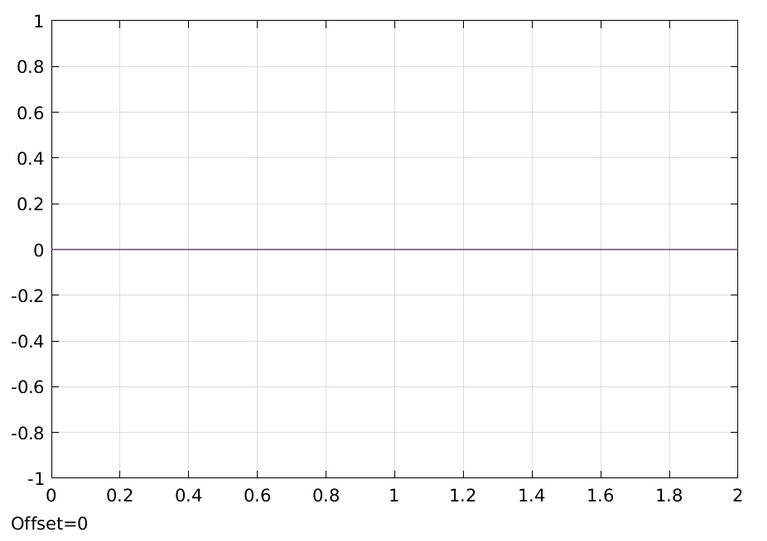
\includegraphics[width=\textwidth]{images/courbe_cas_2_1_TP03.png}
                                        \caption{Etat}
                                        \label{fig3.8.1}
                                \end{subfigure}
                                \hspace{30pt}
                                \begin{subfigure}[b]{0.45\textwidth}
                                        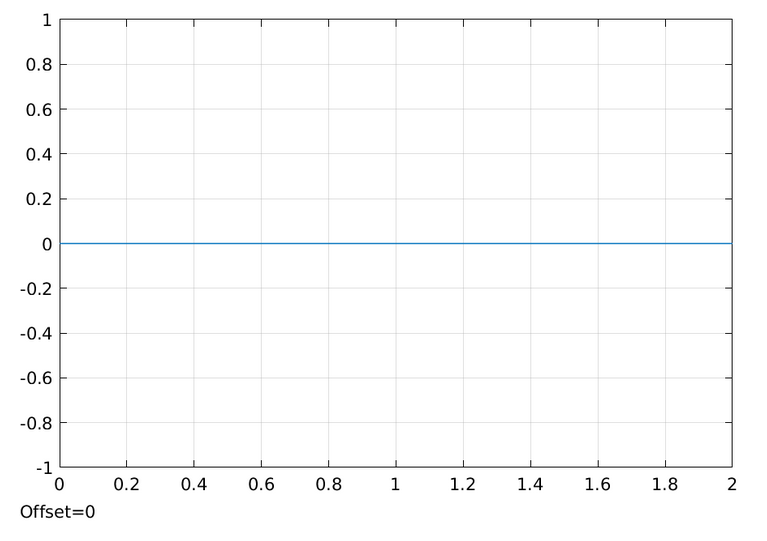
\includegraphics[width=\textwidth]{images/controle_cas_2_1_TP03.png}
                                        \caption{Contrôle}
                                        \label{fig3.8.2}
                                \end{subfigure}
                                \caption{Cas 2.1 avec $x_0=(0,0,0,0)$}
                                \label{fig3.8}
                        \end{figure}

                        \begin{figure}[h!]
                                \centering
                                \begin{subfigure}[b]{0.45\textwidth}
                                        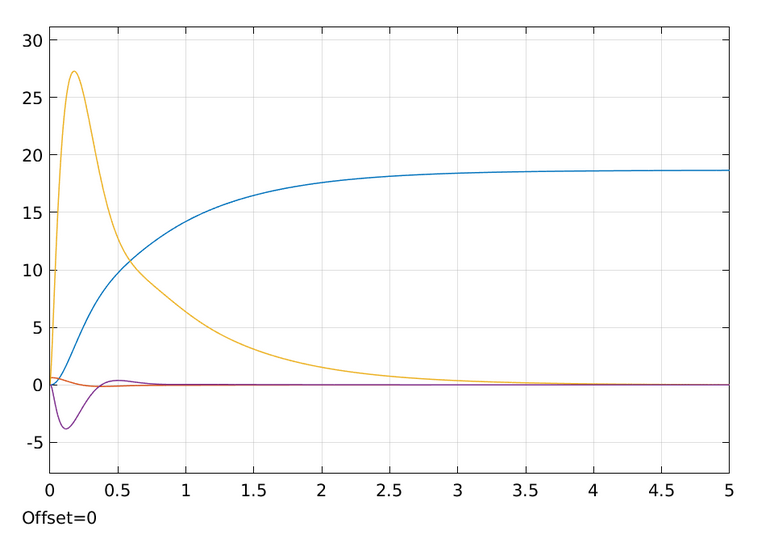
\includegraphics[width=\textwidth]{images/courbe_cas_2_2_TP03.png}
                                        \caption{Etat}
                                        \label{fig3.9.1}
                                \end{subfigure}
                                \hspace{30pt}
                                \begin{subfigure}[b]{0.45\textwidth}
                                        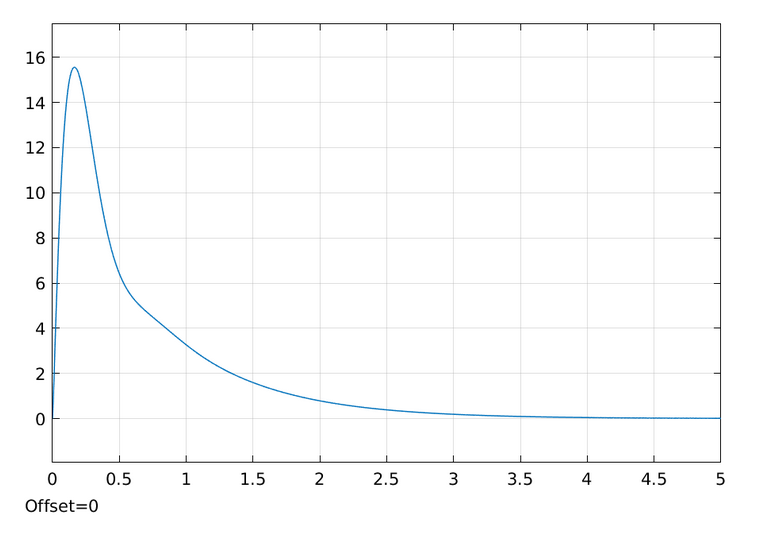
\includegraphics[width=\textwidth]{images/controle_cas_2_2_TP03.png}
                                        \caption{Contrôle}
                                        \label{fig3.9.2}
                                \end{subfigure}
                                \caption{Cas 2.2 avec $x_0=(0,\pi/5,0,0)$}
                                \label{fig3.9}
                        \end{figure}
                        \newpage


                        \begin{figure}[h!]
                                \centering
                                \begin{subfigure}[b]{0.45\textwidth}
                                        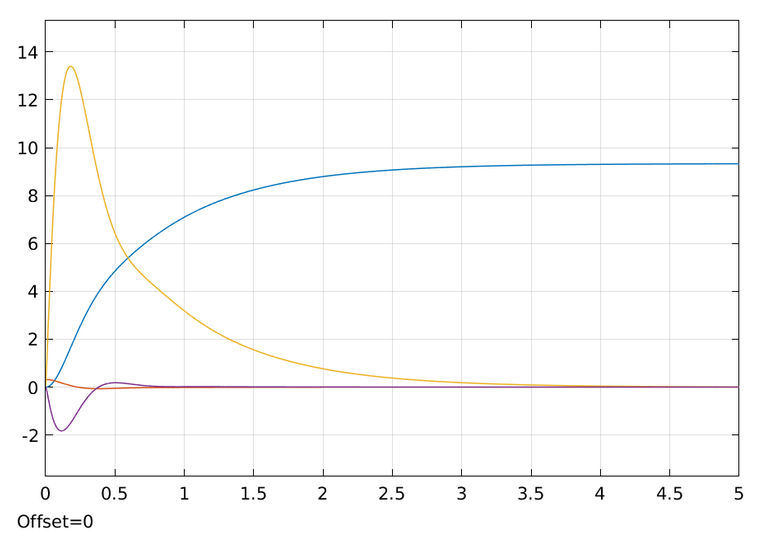
\includegraphics[width=\textwidth]{images/courbe_cas_2_3_TP03.png}
                                        \caption{Etat}
                                        \label{fig3.10.1}
                                \end{subfigure}
                                \hspace{30pt}
                                \begin{subfigure}[b]{0.45\textwidth}
                                        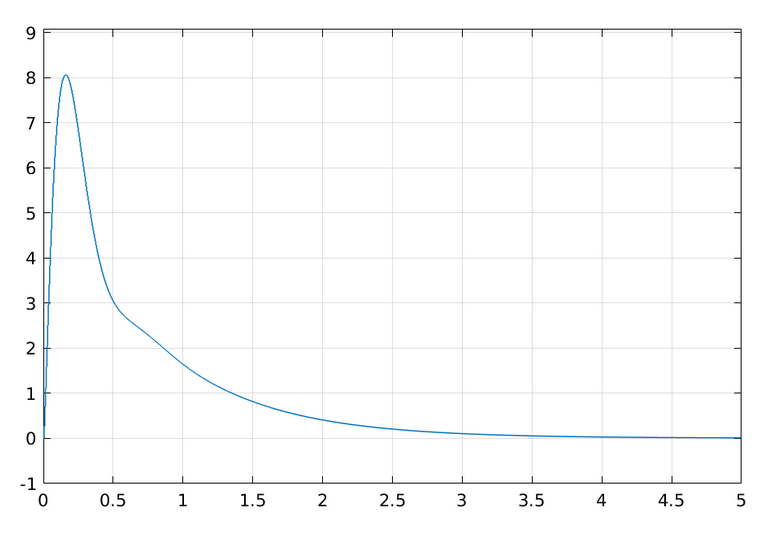
\includegraphics[width=\textwidth]{images/controle_cas_2_3_TP03.png}
                                        \caption{Contrôle}
                                        \label{fig3.10.2}
                                \end{subfigure}
                                \caption{Cas 2.3 avec $x_0=(0,\pi/10,0,0)$}
                                \label{fig3.10}
                        \end{figure}

                        Les allures des différentes courbes sont similaires au cas où l'on considérait le modèle du robot Lego sans capteur ni prédicteur,
                        à la différence de la courbe $\dot \theta$.
                        En effet, pour les cas 2.2 et 2.3 correspondant aux courbes des figures \ref{fig3.9.1} et \ref{fig3.10.1},
                        $\dot \theta$ converge vers une valeur non nulle ($\dot \theta_{\infty} \simeq 18^{°}.s^{-1}$ pour le cas 2.2 et 
                        $\dot \theta_{\infty} \simeq 9^{°}.s^{-1}$ pour le cas 2.3) alors qu'en parallèle, $\dot \psi$ tend vers $0^{°}.s^{-1}$ en régime stationnaire.
                        Cela s'interprète physiquement par le fait qu'une fois le système stabilisé à sa position d'équilibre, ce dernier est en mouvement uniforme
                        dans le sens de la perturbation angulaire initiale.
                        Il ne revient donc pas à un état immobile comme dans le modèle précédent.
                        Cette différence de comportement peut être dû au fait que dans ce modèle, nous avons été obligé de considérer des prédicteurs 
                        (un intégrateur et un dérivateur), qui n'étant pas eux-mêmes des modèles parfaits, induisent des erreurs sur les paramètres de l'état
                        de sortie du système, donc sur la correction du système et en conséquence sur son comportement en régime stationnaire.\\

                        Afin de coller au mieux à la réalité, on ajoute dans le modèle \textsc{Matlab} un bloc \textit{Zero-Order Hold}
                        au niveau du capteur afin que les signaux de sortie de ce dernier soient discrets.
                        On refait tourner le modèle pour les cas 2.1, 2.2 et 2.3 précédents (table 3).
                        
                        \begin{figure}[h!]
                                \centering
                                \begin{subfigure}[b]{0.45\textwidth}
                                        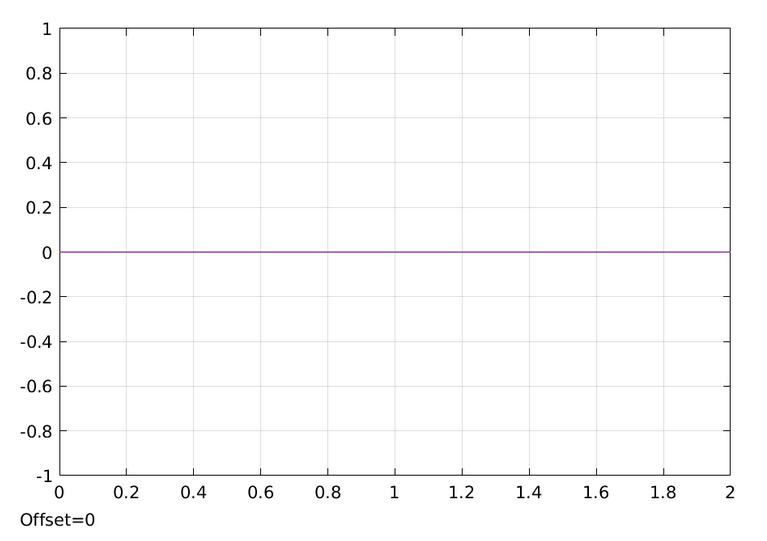
\includegraphics[width=\textwidth]{images/courbe_cas_3_1_TP03.png}
                                        \caption{Etat}
                                        \label{fig3.11.1}
                                \end{subfigure}
                                \hspace{30pt}
                                \begin{subfigure}[b]{0.45\textwidth}
                                        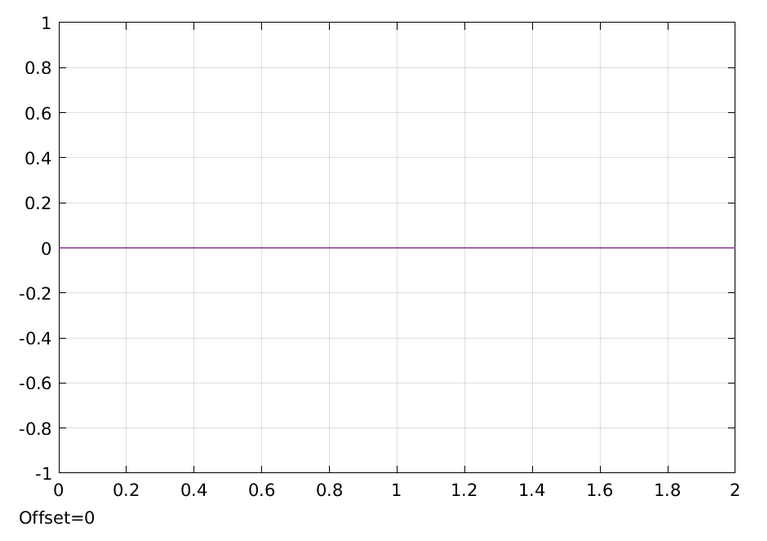
\includegraphics[width=\textwidth]{images/controle_cas_3_1_TP03.png}
                                        \caption{Contrôle}
                                        \label{fig3.11.2}
                                \end{subfigure}
                                \caption{Cas 2.1 avec $x_0=(0,0,0,0)$}
                                \label{fig3.11}
                        \end{figure}

                        \begin{figure}[h!]
                                \centering
                                \begin{subfigure}[b]{0.45\textwidth}
                                        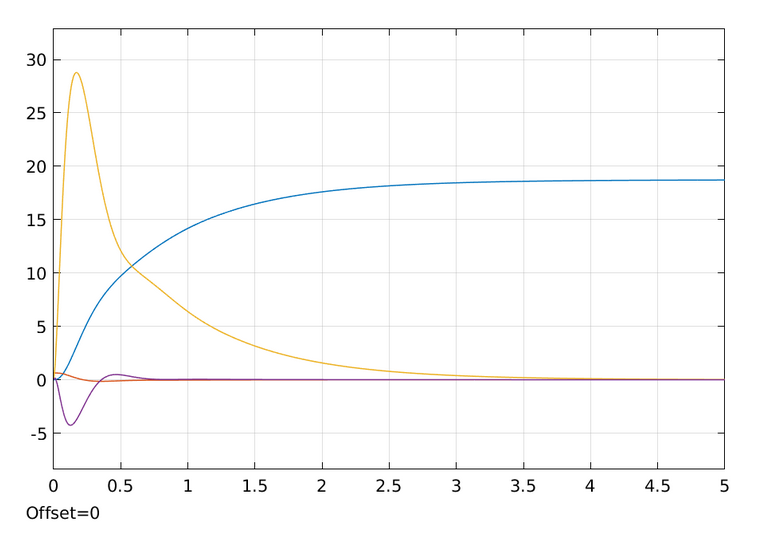
\includegraphics[width=\textwidth]{images/courbe_cas_3_2_TP03.png}
                                        \caption{Etat}
                                        \label{fig3.12.1}
                                \end{subfigure}
                                \hspace{30pt}
                                \begin{subfigure}[b]{0.45\textwidth}
                                        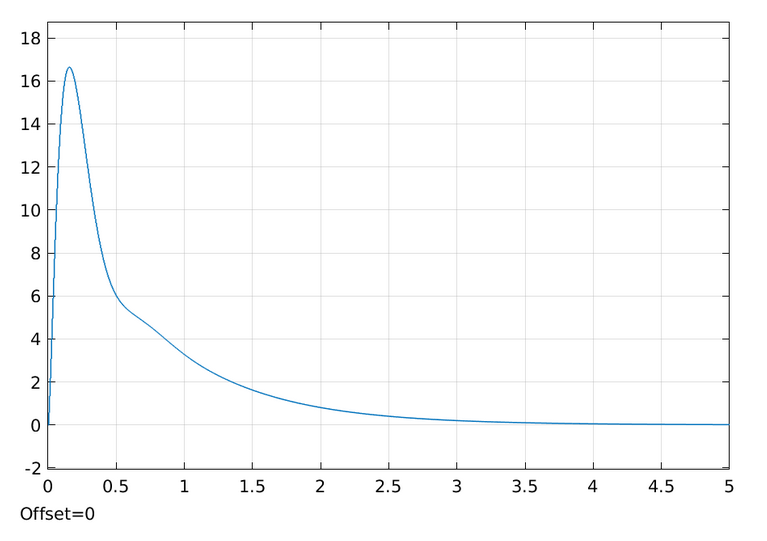
\includegraphics[width=\textwidth]{images/controle_cas_3_2_TP03.png}
                                        \caption{Contrôle}
                                        \label{fig3.12.2}
                                \end{subfigure}
                                \caption{Cas 2.2 avec $x_0=(0,\pi/5,0,0)$}
                                \label{fig3.12}
                        \end{figure}
                        \newpage


                        \begin{figure}[h!]
                                \centering
                                \begin{subfigure}[b]{0.45\textwidth}
                                        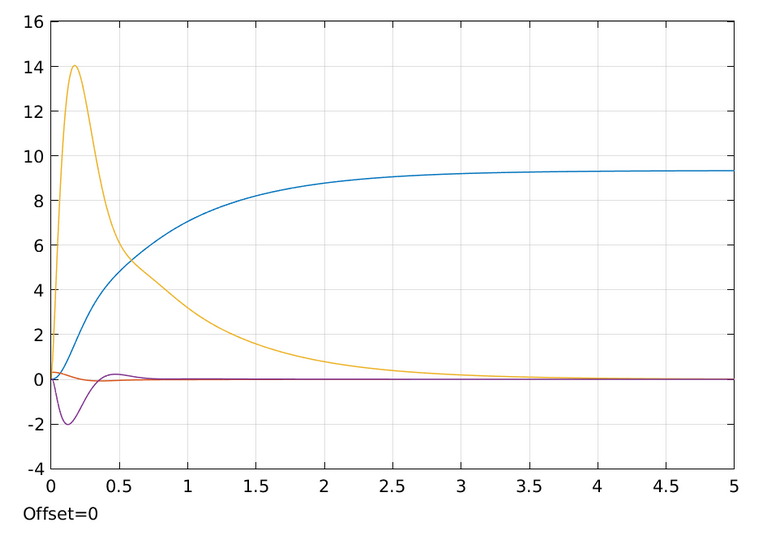
\includegraphics[width=\textwidth]{images/courbe_cas_3_3_TP03.png}
                                        \caption{Etat}
                                        \label{fig3.13.1}
                                \end{subfigure}
                                \hspace{30pt}
                                \begin{subfigure}[b]{0.45\textwidth}
                                        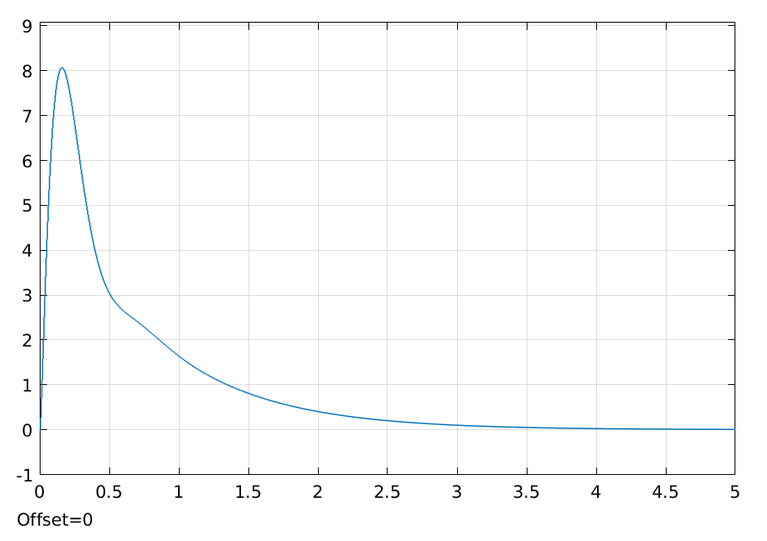
\includegraphics[width=\textwidth]{images/controle_cas_3_3_TP03.png}
                                        \caption{Contrôle}
                                        \label{fig3.13.2}
                                \end{subfigure}
                                \caption{Cas 2.3 avec $x_0=(0,\pi/10,0,0)$}
                                \label{fig3.13}
                        \end{figure}
                        
                        On remarque que ces courbes sont similaires à celles des figures \ref{fig3.8}, \ref{fig3.9} et \ref{fig3.10}.
                        La différence est que certaines des courbes ont des amplitudes légérement supérieures (courbes jaunes des états et courbes bleues des contrôles).
                        On en conclut donc que l'ajout du bloc \textit{Zero-Order Hold} dans \textsc{Matlab} ne modifie que très peu le modèle 
                        qui renvoie toujours des résultats cohérents pour le \textit{Robot Lego Segway}.


        \subsection{Impact des différents paramètres sur la stabilisation du système en boucle fermée (modèle du pendule inversé)}

                \paragraph{Contrôle par retour d'état sans capteur ni prédicteur} 
                
                        Voici les différents cas qui ont été testés lors des TPs :
                        \begin{table}[h!]
                                \centering
                                \begin{tabular}{|c||c|c|c|c|} \hline
                                        \textbf{Cas} & \textbf{$x_0$} & \textbf{$t_f$} & \textbf{$K$} & \textbf{Intégrateur} \\ \hline
                                        Cas 1.1 & $(\pi/20,0)$ & 10 & (30,10) & ode45 \\ \hline
                                        Cas 1.2 & $(\pi/20,0)$ & 100 & (10,1) & ode45 \\ \hline
                                        Cas 1.3 & $(\pi/20,0)$ & 100 & (10,1) & Euler, ode1 \\ \hline
                                        Cas 1.4 & $(\pi/20,0)$ & 1000 & (10,1) & Euler, ode1 \\ \hline
                                        Cas 1.5 & $(\pi/10,0)$ & 100 & (10,1) & ode45 \\ \hline
                                        Cas 1.6 & $(\pi/10,0)$ & 100 & (30,10) & ode45 \\ \hline
                                \end{tabular}
                                \label{table1}
                                \caption{Paramètres de tests pour le retour d'état du pendule inversé sans capteur ni prédicteur}
                        \end{table}


                        \begin{figure}[h!]
                                \centering
                                \begin{subfigure}[b]{0.45\textwidth}
                                        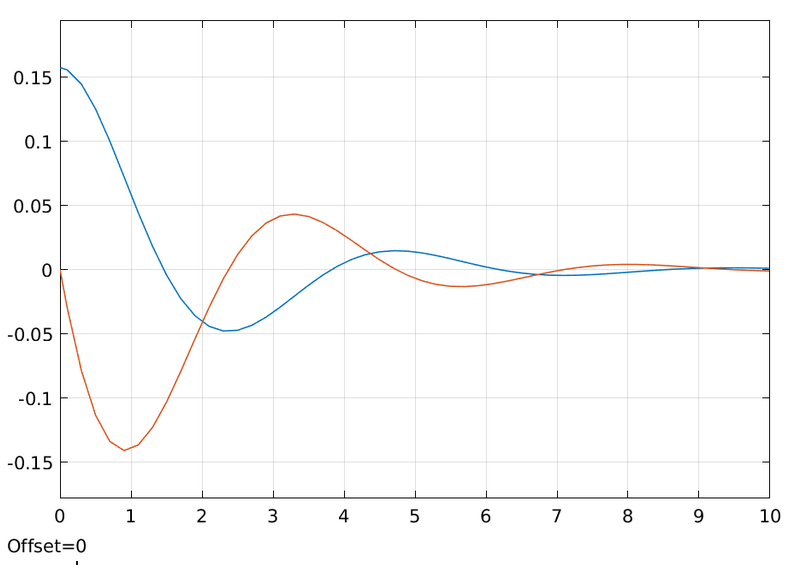
\includegraphics[width=\textwidth]{images/courbe_cas_1_1_TP02.png}
                                        \caption{Etat}
                                        \label{fig_cas_1.1_TP02_etats}
                                \end{subfigure}
                                \hspace{30pt}
                                \begin{subfigure}[b]{0.45\textwidth}
                                        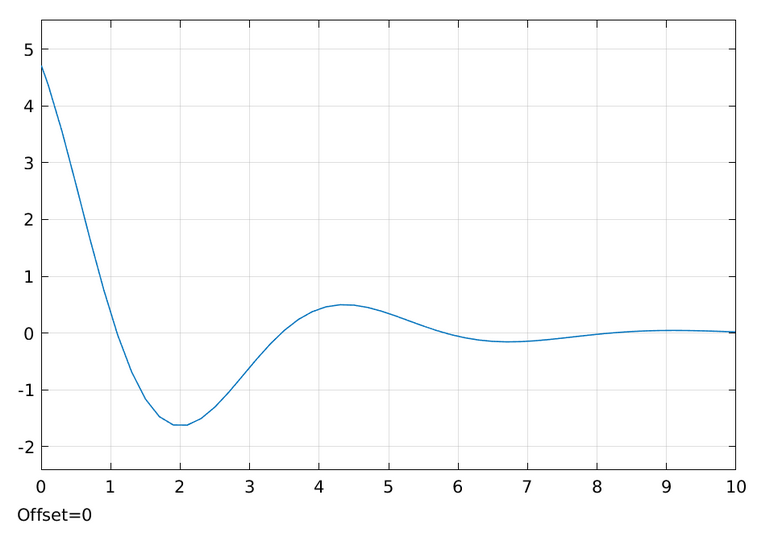
\includegraphics[width=\textwidth]{images/controle_cas_1_1_TP02.png}
                                        \caption{Contrôle}
                                        \label{fig_cas_1.1_TP02_controle}
                                \end{subfigure}
                                \caption{Cas 1.1 TP02}
                                \label{fig_cas_1.1_TP02}
                        \end{figure}

                        \begin{figure}[h!]
                                \centering
                                \begin{subfigure}[b]{0.45\textwidth}
                                        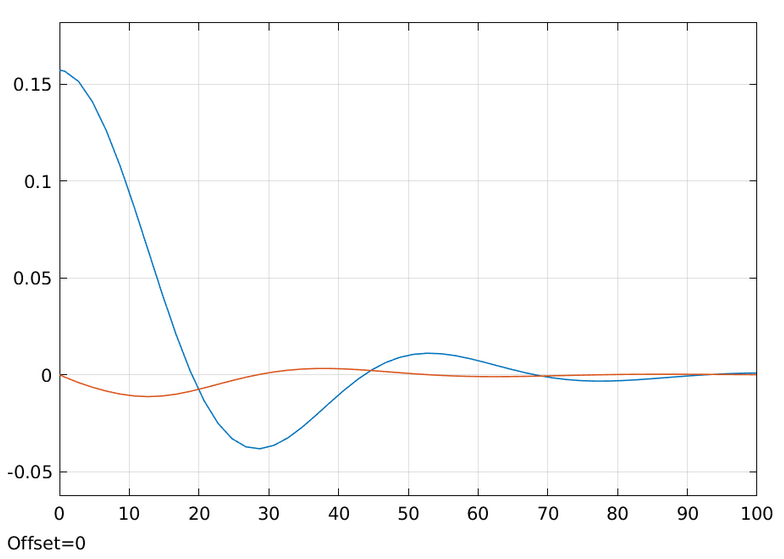
\includegraphics[width=\textwidth]{images/courbe_cas_1_2_TP02.png}
                                        \caption{Etat}
                                        \label{fig_cas_1.2_TP02_etats}
                                \end{subfigure}
                                \hspace{30pt}
                                \begin{subfigure}[b]{0.45\textwidth}
                                        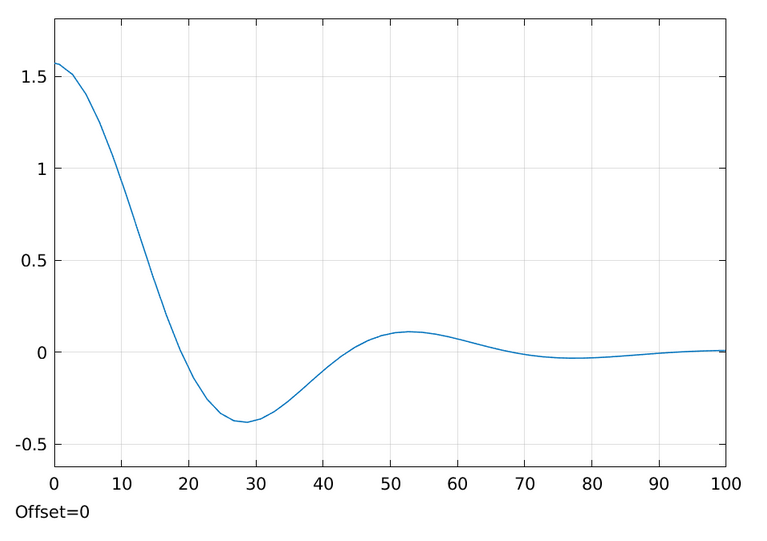
\includegraphics[width=\textwidth]{images/controle_cas_1_2_TP02.png}
                                        \caption{Contrôle}
                                        \label{fig_cas_1.2_TP02_controle}
                                \end{subfigure}
                                \caption{Cas 1.2 TP02}
                                \label{fig_cas_1.2_TP02}
                        \end{figure}

                        On remarque que pour le cas 1.2, où on a fait varier les paramètres de $K$ en prenant $(10,1)$ soit en divisant par un facteur 10
                        par rapport au cas 1.1, le temps de réponse à 5\% est de l'ordre de 10 fois plus long que pour le cas 1.1
                        ($t_{5\%} \simeq 5s$ pour le cas 1.1 et $t_{5\%} \simeq 54s$ pour le cas 1.2).
                        Néanmoins, la différence d'amplitude des oscillations est bien moins notable entre les deux cas
                        ($D_{1\%} \simeq 33\%$ pour le cas 1.1 et $D_{1\%} \simeq 27\%$ pour le cas 1.2). \\

                        On en conclut que la variation des paramètres de $K$ a plus d'influence sur le temps de réponse du système que sur l'amplitude de ses oscillations.
                        En outre, plus les valeurs de $K$ sont grandes, plus le système est rapide. 
                        Néanmoins, il faudrait tester avec d'autres valeurs plus extrêmes pour pouvoir tirer une conclusion sur la dégradation de la stabilité du système.

                        \begin{figure}[h!]
                                \centering
                                \begin{subfigure}[b]{0.45\textwidth}
                                        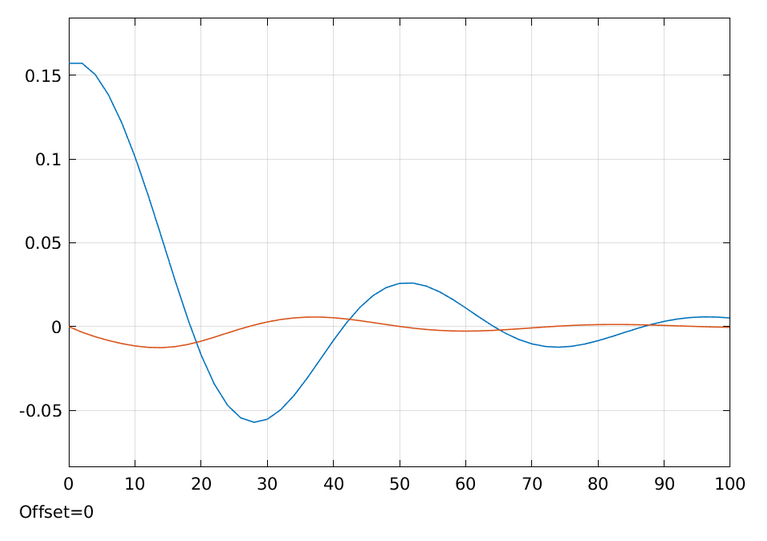
\includegraphics[width=\textwidth]{images/courbe_cas_1_3_TP02.png}
                                        \caption{Etat}
                                        \label{fig_cas_1.3_TP02_etats}
                                \end{subfigure}
                                \hspace{30pt}
                                \begin{subfigure}[b]{0.45\textwidth}
                                        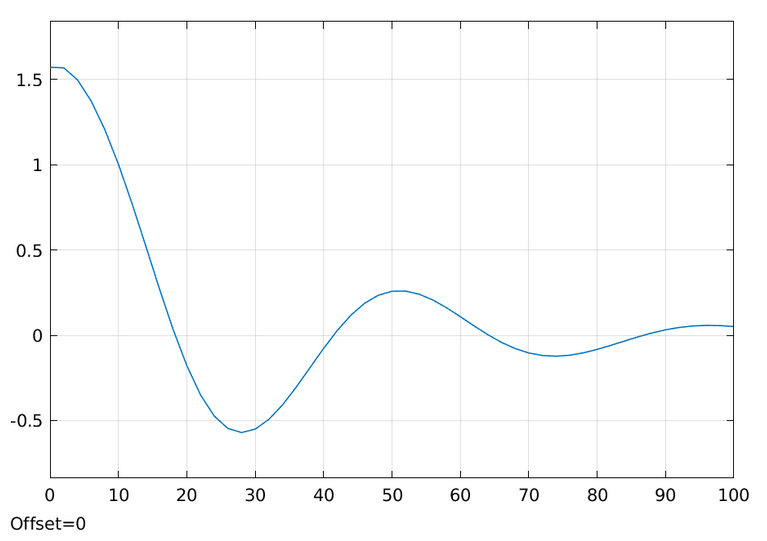
\includegraphics[width=\textwidth]{images/controle_cas_1_3_TP02.png}
                                        \caption{Contrôle}
                                        \label{fig_cas_1.3_TP02_controle}
                                \end{subfigure}
                                \caption{Cas 1.3 TP02}
                                \label{fig_cas_1.3_TP02}
                        \end{figure}

                        \begin{figure}[h!]
                                \centering
                                \begin{subfigure}[b]{0.45\textwidth}
                                        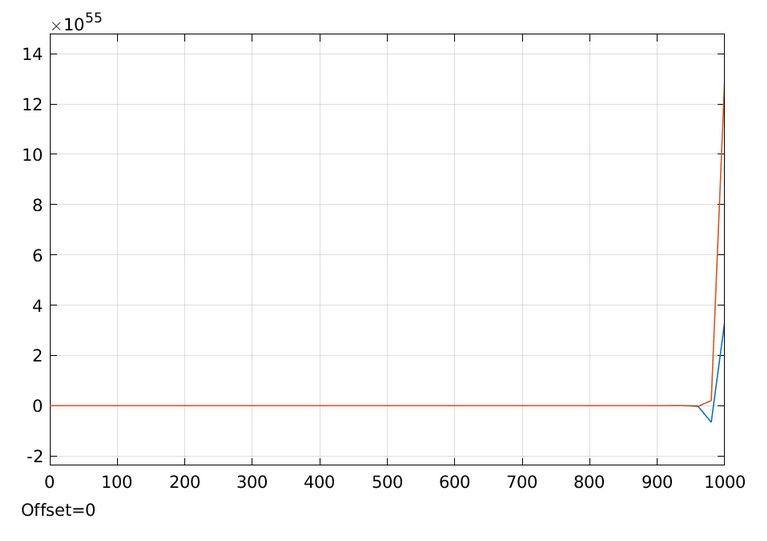
\includegraphics[width=\textwidth]{images/courbe_cas_1_4_TP02.png}
                                        \caption{Etat}
                                        \label{fig_cas_1.4_TP02_etats}
                                \end{subfigure}
                                \hspace{30pt}
                                \begin{subfigure}[b]{0.45\textwidth}
                                        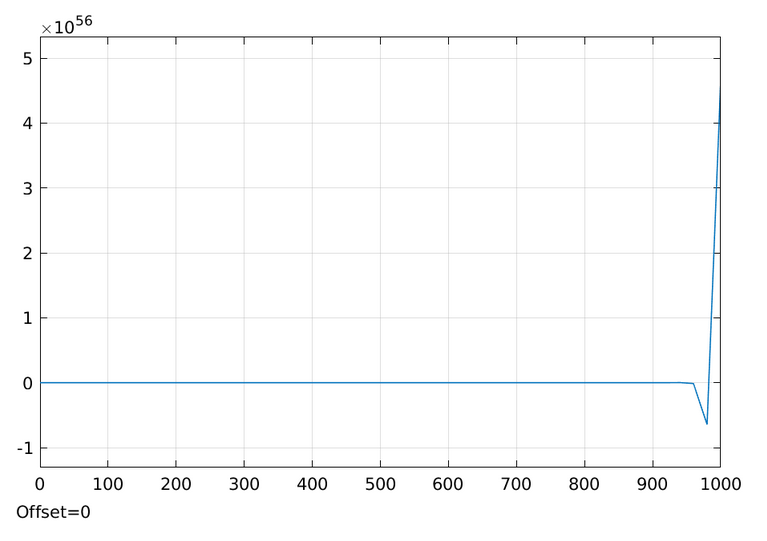
\includegraphics[width=\textwidth]{images/controle_cas_1_4_TP02.png}
                                        \caption{Contrôle}
                                        \label{fig_cas_1.4_TP02_controle}
                                \end{subfigure}
                                \caption{Cas 1.4 TP02}
                                \label{fig_cas_1.4_TP02}
                        \end{figure}

                        Les cas 1.3 et 1.4 sont similaires au cas 1.2 au niveau des choix des paramètres (position initiale $x_0$ et valeur de $K$)
                        mais le choix du résolveur de l'équation différentielle globale du système diffère (Euleur, Ode1).
                        Ils servent alors à nous montrer dans quelle mesure le résolveur et le pas de discrétisation du temps impactent le résultat. \\

                        Pour le cas 1.3, on a fixé la discrétisation du temps et on a fait tourner la simulation sur une durée de $100s$.
                        On remarque que le résultat obtenu diffère déjà par rapport à celui obtenu pour le cas 1.2.
                        En effet, le temps de réponse est plus long ainsi que l'amplitude des oscillations ($t_{5\%} \simeq 80s$ et $D_{1\%} \simeq 40\%$).
                        On peut donc penser que pour les mêmes paramètres fixés, la stabilité et le temps de réponse du système se sont dégradés.
                        Ce qui nous induit en erreur. \\
                        
                        Pour le cas 1.4, cette incohérence se voit justifiée puisque pour une même discrétisation temporelle, 
                        (\textit{i.e.} même nombre de pas temporels que le cas précédent) mais pour un temps de simulation de $1000s$,
                        les résultats obtenus deviennent complètement incohérents et ne traduisent plus du tout le comportement réel du système.

                        \begin{figure}[h!]
                                \centering
                                \begin{subfigure}[b]{0.45\textwidth}
                                        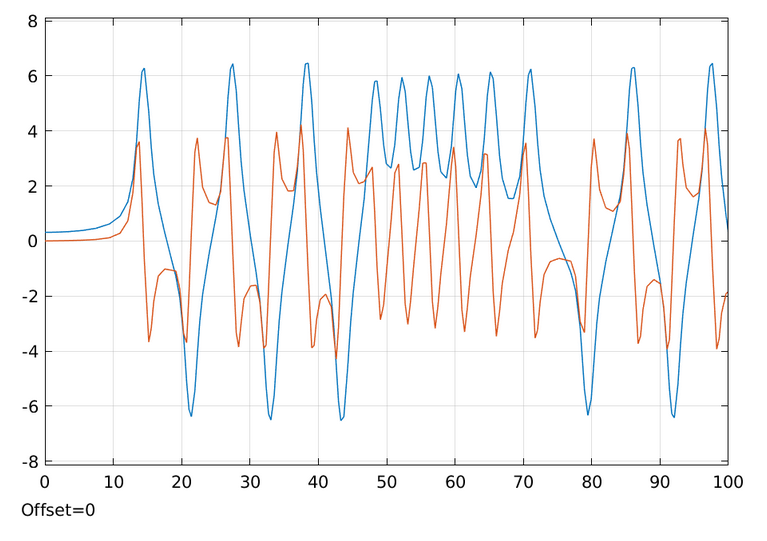
\includegraphics[width=\textwidth]{images/courbe_cas_1_5_TP02.png}
                                        \caption{Etat}
                                        \label{fig_cas_1.5_TP02_etats}
                                \end{subfigure}
                                \hspace{30pt}
                                \begin{subfigure}[b]{0.45\textwidth}
                                        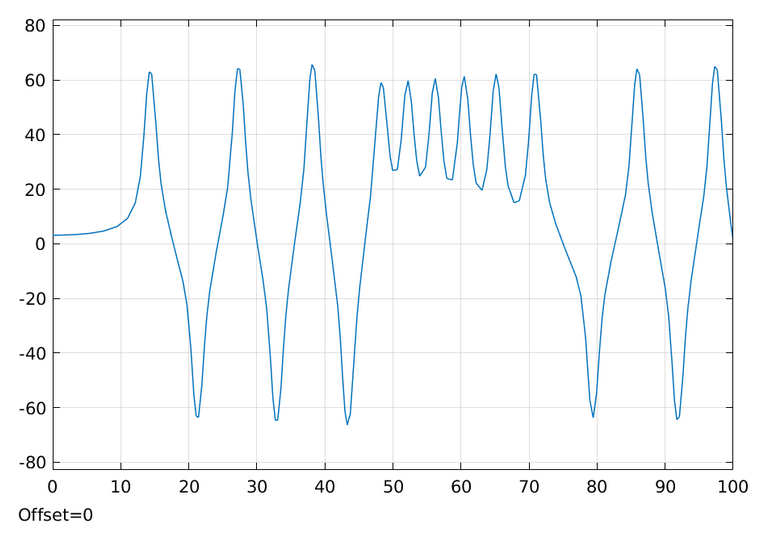
\includegraphics[width=\textwidth]{images/controle_cas_1_5_TP02.png}
                                        \caption{Contrôle}
                                        \label{fig_cas_1.5_TP02_controle}
                                \end{subfigure}
                                \caption{Cas 1.5 TP02}
                                \label{fig_cas_1.5_TP02}
                        \end{figure}

                        \begin{figure}[h!]
                                \centering
                                \begin{subfigure}[b]{0.45\textwidth}
                                        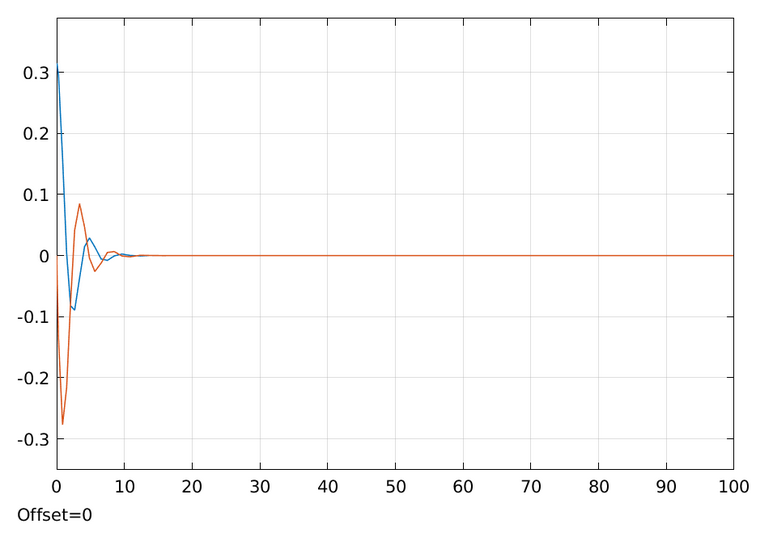
\includegraphics[width=\textwidth]{images/courbe_cas_1_6_TP02.png}
                                        \caption{Etat}
                                        \label{fig_cas_1.6_TP02_etats}
                                \end{subfigure}
                                \hspace{30pt}
                                \begin{subfigure}[b]{0.45\textwidth}
                                        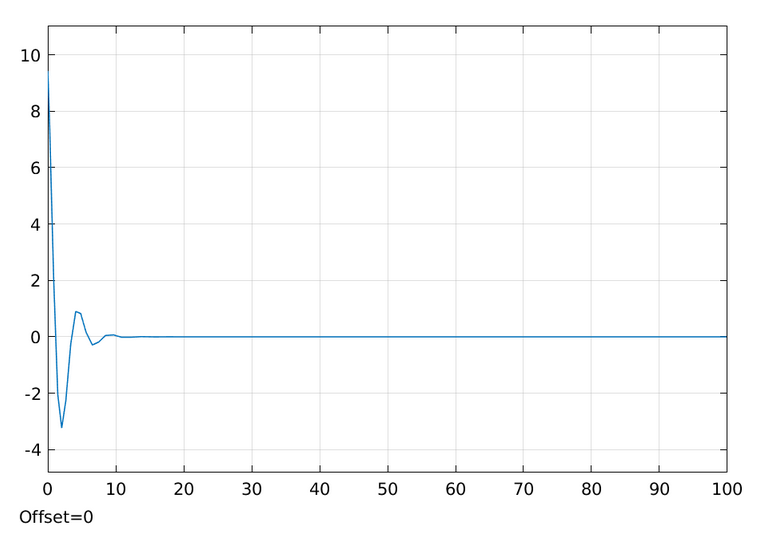
\includegraphics[width=\textwidth]{images/controle_cas_1_6_TP02.png}
                                        \caption{Contrôle}
                                        \label{fig_cas_1.6_TP02_controle}
                                \end{subfigure}
                                \caption{Cas 1.6 TP02}
                                \label{fig_cas_1.6_TP02}
                        \end{figure}

                        Les cas 1.5 et 1.6 servent à nous montrer l'influence du réglage du correcteur pour une perturbation initiale de l'angle plus importante.
                        En effet, on prend dans les deux cas comme valeur initiale $x_0 = (\pi/10, 0)$. \\

                        Pour le cas 1.4, on remarque que pour les valeurs $(10,1)$ des paramètres de $K$ choisis, le système devient instable.
                        En effet, les valeurs de $\theta$ et $\dot \theta$ croîssent pour atteindre les valeurs maximumales en valeur absolue 
                        d'environ 6 rad et 4 rad.$s^{-1}$.
                        Cela signifie que le pendule inversé effectue un tour complet pour atteindre sa position d'équilibre avant de repartir
                        dans l'autre sens et ainsi de suite.
                        Transposé au cas réel du robot Lego où l'angle ne pourra pas dépasser l'intervalle $\left[ -\frac{\pi}{2} ; \frac{\pi}{2} \right]$,
                        le système ne sera pas stabilisé et se retrouvera par terre. \\

                        Pour le cas 1.5, on remarque que pour les valeurs $(30,10)$ des paramètres de $K$ choisis, le système arrive à se 
                        stabiliser asymptotiquement autour de sa position d'équilibre. \\

                        On en conclut donc qu'il vaut mieux choisir les valeurs des paramètres de $K$ de façon à assurer 
                        la stabilité du système pour une plage de position angulaire initiale optimale.


        \section{Conclusion}

                \hspace{20pt} Pour conclure, cette étude de cas sur le pendule inversé puis sur le robot Lego en pendule inversé nous aura appris des bases de l'automatique.
                Ainsi, nous avons abordé des notions fondamentales telles que la stabilisation d'un système avec un contrôle par retour d'état
                qu'il comporte un ensemble de capteurs et de prédicteurs ou non.


        \newpage
        \section{Annexes}

                \subsection{Equations du modèles du Robot Lego}
                \label{equations_robot_lego}

                        $$
                        \begin{cases}
                                \ddot \theta = \frac{C_4 C_3 - C_2 C_5 + C_4 C_{\theta} (U(t), \dot \theta (t), \dot \psi (t)) - C_2 C_{\psi} (U(t), \dot \theta (t), \dot \psi (t))}{C_4 C_1 - C_2^2} \\
                                \ddot \psi = \frac{C_{\psi} (U(t), \dot \theta (t), \dot \psi (t)) - C_2 \ddot \theta - C_5}{C_4}
                        \end{cases}
                        $$

                        Avec les expressions des différentes inerties $C_{i \in \llbracket 1,5 \rrbracket}$ en $kg.m^2$ :
                        \begin{itemize}
                                \item $C_1 = (2m + M)R^2 + 2J_W + 2n^2 J_m$
                                \item $C_2 = MLR - \cos (\psi) - 2n^2 J_m$
                                \item $C_3 = -MLR \dot \psi^2 \sin (\psi)$
                                \item $C_4 = ML^2 + J_{\psi} + 2n^2 J_m$
                                \item $C_5 = -MgL \sin (\psi)$
                        \end{itemize}

                        Avec également $C_{\theta} (U(t), \dot \theta (t), \dot \psi (t))$ et $C_{\psi} (U(t), \dot \theta (t), \dot \psi (t))$
                        qui sont les expressions respectives des couples (en N.m) sur l'axe de rotation au point $O$ et au point $M$ du
                        schéma cinématique de la figure \ref{fig_robot_lego} :
                        \begin{itemize}
                                \item $C_{\theta} (U(t), \dot \theta (t), \dot \psi (t)) = \frac{2K_t U(t)}{R_m} - 2 \left( \frac{K_t K_b}{R_m} + f_m + f_w \right) \dot \theta + 2 \left( \frac{K_t K_b}{R_m} + f_m \right) \dot \psi$
                                \item $C_{\psi} (U(t), \dot \theta (t), \dot \psi (t)) = - \frac{2K_t U(t)}{R_m} - 2 \left( \frac{K_t K_b}{R_m} + f_m + f_w \right) \dot \theta + 2 \left( \frac{K_t K_b}{R_m} + f_m \right) \dot \psi$
                        \end{itemize}
                        où :
                        \begin{itemize}
                                \item $g$ la constante de gravitation terrestre en $m.s^{-2}$
                                \item $m$ la masse d'une roue en $kg$
                                \item $R$ le diamètre de la roue en $m$
                                \item $J_W$ l'inertie de la roue en $kg.m^2$
                                \item $M$ la masse du corps du Robot en $kg$
                                \item $H$ la hauteur du Robot en $m$
                                \item $L=\frac{H}{2}$ la distance entre l'axe de rotation de la roue et le centre de masse du système en $m$
                                \item $J_{\psi} = \frac{ML^2}{3}$ l'inertie du corps du Robot qui est assimilé à un cylindre en $kg.m^2$
                                \item $J_m$ l'inertie du rotor du moteur en $kg.m^2$
                                \item $R_m$ la résistance interne du moteur en $\Omega$
                                \item $K_b$ la constante électrique du moteur en $V.s.rad^{-1}$
                                \item $K_t$ la constante mécanique du moteur en $N.m.A^{-1}$
                                \item $n$ le rapport de transmission entre le moteur et la roue
                                \item $f_m$ le coefficient de frottement entre le corps du Robot et le moteur en $N.m.s$
                                \item $f_W$ le coefficient de frottement entre la roue et le sol en $N.m.s$
                        \end{itemize}


                \subsection{Code}

                        \hspace{25pt} Afin d'observer notre modèle de simulation sur le système réel du \textit{Robot Lego Segway}, nous avons implémenté le modèle du robot Lego
                        pendule inversé en C au travers du code suivant. Nous avons utilisé la méthode des rectangles de Riemann pour l'intégration discrète et 
                        des développements limités pour la dérivation discrète.

                        \begin{minted}[linenos]{c}
#include "tpl_os.h"
#include "nxt_motors.h"
#include "ecrobot_interface.h" 
#include "ecrobot_private.h"
#include "math.h"
#include "tools.h"    
#include "nxt_config.h"         

/* ------------------------------------------------------------------------ */
/*  Fonctions de configuration OSEK                                         */
/* ------------------------------------------------------------------------ */
FUNC(int, OS_APPL_CODE) main(void)
{   
StartOS(OSDEFAULTAPPMODE);
return 0;
}

DeclareTask(pendule);
DeclareTask(affichage);

DeclareAlarm(alarm_pendule);
DeclareAlarm(alarm_affichage);

/* ------------------------------------------------------------------------- */
/* Variables globales du système                                             */
/* ------------------------------------------------------------------------- */

/* Gyro calibration */
int  gyro_offset;                   /* gyroscope sensor offset value(deg)    */
int  gyro_offset_sum;               /* sum of gyroscope sensor offset 
                                value(deg)                            */
int  avg_cnt;                       /* average count to calculate 
                                gyro offset                           */

float xe[4] = {0.0,0.0,0.0,0.0};    /* equilibrium state                     */
float ue    = 0.0;                  /* command at equilibrium                */
float x[4];                         /* state                                 */
float y[2];                         /* observations                          */
float u;                            /* command of the controller (V)         */
float setpoint;                     /* target value for theta variable       */
float dt;

typedef enum {
INIT_MODE,      /* system initialize mode */
CAL_MODE,       /* gyro sensor offset calibration mode */
CONTROL_MODE    /* balance and RC control mode */
} MODE_ENUM;
MODE_ENUM nxtSegway_mode= INIT_MODE;



void controller () {
const float K[4] = {0.6700, 19.9053, 1.0747, 1.9614};
u = ue;
for (int i = 0; i<4; i++) {
u += K[i] * (x[i] - xe[i]);
}
}

void estimateur () {
float theta;

// d(psi)/dt -> d(psi)/dt
x[3] = y[1];

// d(psi)/dt -> psi
// On utilise la methode des rectangles
x[1] = x[3] * dt + x[1];

//theta = thetam + psi
theta = y[0] + x[1];

//theta -> d(theta)/dt
x[2] = (theta - x[0])/dt;
x[0] = theta;

}


TASK(pendule) {

int initial_time= 0;
        
switch(nxtSegway_mode){

case(INIT_MODE):

nxt_motor_set_count(PORT_MOTOR_L, 0);   /* reset left motor count         */
nxt_motor_set_count(PORT_MOTOR_R, 0);   /* reset right motor count        */

/* Initial state */
for(int i=0;i<4;i++){
x[i] = xe[i];
}

/* target value */
setpoint            = xe[0];

initial_time= ecrobot_get_systick_ms();
init_time(initial_time);

/* Gyro calibration */
gyro_offset         = 0;
gyro_offset_sum     = 0;
avg_cnt             = 0;

nxtSegway_mode = CAL_MODE;

break;

case(CAL_MODE):

gyro_offset_sum += (int) ecrobot_get_gyro_sensor(PORT_GYRO); 
/* accumulation of the values given by the gyro */

avg_cnt++;

if ((ecrobot_get_systick_ms() - initial_time) >= 1500) {
gyro_offset = gyro_offset_sum / avg_cnt;
/* mean of the previous measures */

ecrobot_sound_tone(440, 500, 30);       /* beep a tone                 */
nxtSegway_mode = CONTROL_MODE;
}

break;

case(CONTROL_MODE):

y[0] = getMotorAngle();
y[1] = getGyro(gyro_offset);
dt = delta_t();
estimateur();
controller();
nxt_motors_set_command(u);

break;

default:
/* unexpected mode */
nxt_motor_set_speed(PORT_MOTOR_L, 0, 1);
nxt_motor_set_speed(PORT_MOTOR_R, 0, 1);
break;
}
TerminateTask();
}


TASK(affichage) {
/*display informations*/
display_clear(0);

//disp(1, " PWM  = ", (int)(pwmR+pwmL)/2);
disp(2, " y[0] = ", (int)(y[0]*RAD2DEG));
disp(3, " y[1] = ", (int)(y[1]*RAD2DEG));
disp(4, " x[0] = ", (int)((x[0]) * RAD2DEG));
disp(5, " x[1] = ", (int)((x[1]) * RAD2DEG));
disp(6, " x[2] = ", (int)((x[2]) * RAD2DEG));
disp(7, " x[3] = ", (int)((x[3]) * RAD2DEG));

TerminateTask();
}

ISR(isr_button_start)
{
ecrobot_status_monitor("isr_button_start");

}

ISR(isr_button_stop)
{
ShutdownOS(E_OK);
}

ISR(isr_button_left)
{
ecrobot_status_monitor("isr_button_left"); 

}

ISR(isr_button_right)
{
ecrobot_status_monitor("isr_button_right");   

}

        \end{minted}

\end{document}